\documentclass[12pt, letterpaper]{article}
\usepackage[utf8]{inputenc}
\usepackage[margin=1in]{geometry}
\usepackage[super]{nth}

\usepackage{lineno}
\usepackage[
singlelinecheck=false
]{caption}
\usepackage{amsmath}
\usepackage{amsfonts}
%\usepackage{bm}
%\usepackage{bbm}
\usepackage{graphicx}
\usepackage{csvsimple}
%\usepackage[section]{placeins}
\usepackage{lineno}
\usepackage{natbib}
\usepackage[T1]{fontenc}
\usepackage[breaklinks]{hyperref}
%\usepackage{microtype}

\title{Estimating F-statistics in a probabilistic PCA space}
\author{Divyaratan Popli, Benjamin M. Peter}
%\date{5 August 2021}
\linenumbers

\setlength{\parskip}{1em}
\setlength{\parindent}{0em}

\newcommand{\BZ}{\mathbf{Z}}
\newcommand{\BD}{\mathbf{D}}
\newcommand{\BN}{\mathbf{N}}
\newcommand{\BH}{\mathbf{H}}
\newcommand{\BP}{\mathbb{P}}
\newcommand{\Btheta}{\pmb{\theta}}


\newcommand{\MX}{\mathbf{X}}
\newcommand{\MS}{\mathbf{S}}
\newcommand{\MP}{\mathbf{P}}
\newcommand{\MG}{\mathbf{G}}
\newcommand{\MZ}{\mathbf{Z}}
\newcommand{\ML}{\mathbf{L}}
\newcommand{\COV}[2]{\text{Cov}(#1,#2)}

\newcommand{\CX}{\mathcal{X}}


\hbadness=99999

\usepackage{breqn}

\begin{document}

\maketitle


\begin{abstract}

\noindent Principal component analysis (PCA) and $F$-statistics are routinely used in population genetic and archaeogenetic studies. However, these are closely related analyses and reveal the same biological signal. Here, we present a statistical framework to combine them into a joint analysis. In particular, we discuss the differences of probabilistic PCA, Latent Subspace Estimation and ordinary PCA, and show that $F$-statistics are more naturally interpreted in a probabilistic PCA framework. We also show that individual-based $F$-statistics can be accurately estimated from probabilistic PCA in the presence of large amounts of missing data. We compare estimates from probabilistic PCA-based framework to ADMIXTOOLS 2 using simulations and published data, and show that this joint estimation framework addresses limitations of estimating F-statistics and PCA  independently.

\end{abstract}

\section{Introduction}
Many populations live in heterogeneous and changing environments, and thus will exhibit some population structure, which we expect to change over time. Over short time scales, the two principal forces affecting this structure are drift (which creates differentiation between populations over time due to isolation), and admixture (secondary contact between isolated populations), that causes intermediate genotypes. A common goal is to characterize the genetic variation caused by these processes.

In particular for humans, there has been a long-standing debate on how we define genetic population structure, whether populations as such exist, and to what degree they are the result of biased sampling designs \cite{serre_evidence_2004, rosenberg_clines_2005, peter_genetic_2020}, and how they affect ancestry estimation \cite{mathieson_what_2020, simon_contribution_2023}.

Questions like these are of fundamental importance because they impact how we assess access to genetic medicine, how we think about racial discriminations and other (mis)uses of genetic variation.


Admixture between previously isolated populations is common in nature, and affects the patterns of genetic diversity. From these patterns of genetic diversity, one can reconstruct the past events of admixture.  

\subsection{Overview of methods to study admixture}
There are several methods available to make inferences about population structure arising from many diverse processes including geographical isolation, migration, admixture and founder events, that explain the observed genetic diversity. \cite{schraiber_methods_2015}.


These methods can be classified as local or global ancestry based. Local ancestry based methods infer ancestry at each locus and reveal recent history of each individual, but have low power to infer events in deep past \cite{vi_genome-wide_2023, brisbin_pcadmix_2012, price_sensitive_2009, sankararaman_estimating_2008}. Global ancestry methods focus on estimating the allele frequencies in ancestral populations, as well as the ancestry proportion of each individual \cite{pritchard_inference_2000, gopalan_scaling_2016, noauthor_ancient_nodate,alexander_fast_2009, tang_estimation_2005}. Principal Component Analysis (PCA) is a widely used global ancestry method used to uncover population structure \cite{mcvean_genealogical_2009, engelhardt_analysis_2010}. PCA tends to cluster similar individuals nearby, and provides a an easy to understand and often useful visualization of the genetic variation in the data. The big caveat is that it can be difficult to interpret a PCA plot since it does not provide model comparison or a formal test of admixture \cite{novembre stevens 2008 nature, degiorgio_geographic_2013}.   

%\subsection{F-statistics}
A popular way to quantify drift and admixture relies on a set of statistics called $F$-statistics \cite{patterson_ancient_2012, peter_admixture_2016}. $F$-statistics are particularly in wide use in applications of ancient human population structure \cite{orlando_ancient_2021}. 

They provide an intuitive and powerful way to test hypothesis of admixture by measuring the genetic drift shared between two, three, or four populations \cite{patterson_ancient_2012, peter_admixture_2016}. Based on these measures of genetic drift, one can formulate hypotheses of admixture or population history. In this framework, the null model is represented by a tree connecting the populations (Fig. \ref{fig2:overview}). A tree model does not allow for gene flow between populations, and thus admixture would lead to rejection of the null model. 


\subsection{Estimation of F-statistics}\label{intro-fstats-estimation}

As we will define in full detail in the theory section, $F$-statistics are defined in terms of population allele frequencies at a large number of loci. Population allele frequencies are different from the sample allele frequencies that we can obtain from data. Patterson et al showed that a naive estimator would be biased, and introduced a bias-correction term . This bias is largest if the sample size is small (e.g. for single genomes), and will reduce in magnitude for larger samples. 

Thus, from a statistical perspective, it would make sense to group samples into as large groups as possible, because this improves the statistical accuracy. However, on the flip side,  many species with distributions over large ranges, are not easily subdivided into discrete populations. Treating each individual independently will lead to an accurate description of the overall, genetic structure, but will be hard to interpret and will have low statistical accuracy. On the flip side, grouping as many individuals together as possible improves statistical accuracy, but increase the danger of an overly  simplistic view of human genetic structure.


\subsubsection{Missing data}
The amount of preserved DNA is often a limiting factor of ancient DNA data, and hence low-coverage and of heterogeneous data quality are common issues in data analysis  \cite{orlando_ancient_2021}. In this case, missingness can make individual-based statistics even harder to estimate. We discuss the issue of missingness in detail in section XX.

Here, we aim to address these issues by developing a framework to jointly estimate F-statistics in a framework that does not require a priori assignment of individuals to discrete populations, and is much more robust to data missing at random.


\subsection{PCA}
The key ingredient in our approach is PCA. There are several ways to motivate PCA; here we think of PCA is a dimensionality reduction technique used to transform a high-dimensional data set into a lower-dimensional representation, while retaining as much of the original variation in the data as possible. PCA achieves this by finding orthogonal axes, called principal components (PCs), that capture the maximum variance in the data. It is commonly used to understand structure and admixture between populations \cite{patterson_population_2006,novembre_genes_2008,noauthor_cavalli-sforza_nodate,mcvean_genealogical_2009,brisbin_pcadmix_2012}. 

PCA was introduced and popularized as a tool to study human genetic structure by Cavalli-Sforza et al., and using just a handful of genetic loci, they was able to use PCA to accurately describe patterns of human genetic variation, and to make inference about their possible causes, although the way these patterns were analyzed were typically qualitative \cite{menozzi_synthetic_1978, sforza_great_1995, noauthor_cavalli-sforza_nodate}.

As is still the norm with $F$-statistics, Cavalli-Sforza aggregated individuals into populations before performing PCA. With the advent of genomic data, his methods became superseded by individual-based approaches, which addressed many of the issues about grouping individuals we discussed above \cite{patterson_population_2006, novembre_genes_2008, price_principal_2006}.

\subsection{Probabilistic PCA and Latent Subspace Estimation (LSE)}

Probabilistic PCA (PPCA) is an extension of PCA that incorporates a probabilistic framework \cite{tipping_probabilistic_nodate}. PPCA models the observed data as generated by a linear transformation of a lower-dimensional latent space $\mathbf{W}$ with added Gaussian noise $\Psi$. 
The key idea of adding noise is that we aim to separate the variation caused by the population structure that we are ultimately interested in, and which is modeled by $W$, from the variation caused by the estimation of the population allele frequencies from sample allele frequencies (modelled by $Psi$).


A similar approach to model the observed data is Latent Subspace Estimation (LSE) \cite{cabreros_likelihood-free_2019}. Similar to PPCA, a latent space $\mathbf{W}$ models the relationships between individuals, but the  sample allele frequencies are modelled as independent, binomially distributed random variable for each individual \cite{van_waaij_evaluation_2023, cabreros_likelihood-free_2019, chen_consistent_2015}. We give a detailed description of both frameworks in sections \ref{theory-ppca} and \ref{theory-lse}. In practice, the main different between PCA, PPCA and LSE is how they model the noise in the observed data due to sampling (see Fig.\ref{fig1:pca_ppca}). 

\begin{figure}[ht!]
    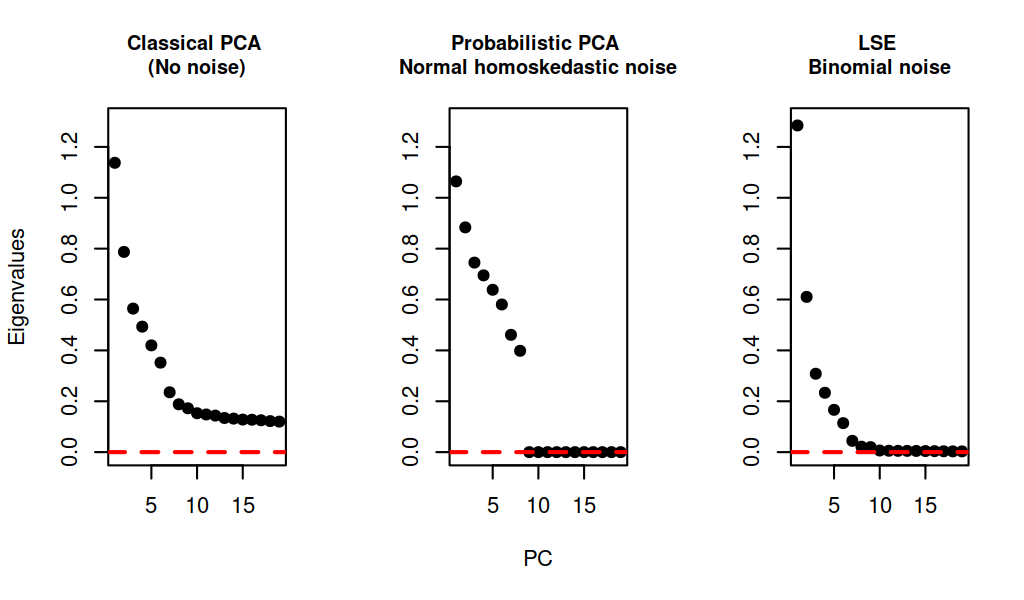
\includegraphics[width=16.5cm]{plots/pca_all_genetic.png}
    \centering
    \caption{Comparison of PCA, PPCA and LSE: We simulated genotypes of 10 populations with 10 individuals each, and compared the top eigenvalues obtained from different PCA methods.}
    \label{fig1:pca_ppca} 
\end{figure}

\subsection{PCA and $F$-statistics}
A common analysis paradigm in ancient DNA is to use PCA for exploratory and descriptive analyses, and then follow them up with methods based on $F$-statistic for a more formal treatment (typically in a third step, methods that synthesize many $F$-statistics are also applied, although we will not cover those here). Because they were developed independently and occur at different stages of the analyses, PCA and F-statistics use different data groupings and different normalizations, and are usually not directly compared. 

Recently, we showed that the information contained in $F$-statistics and PCA is closely related, and that $F$-statistics can be interpreted geometrically in the context of PCA \cite{peter_geometric_2022, oteo-garcia_geometrical_2021}.

Using these frameworks, we showed that genetic drift will move individuals further apart from each other on a PCA-plot. Independent drift, i.e. unconnected populations, will drift on orthogonal axes in PCA-space. On the other hand, admixted individuals will be placed between their populations of origin.  


However, while \cite{peter_geometric_2022} develops a theoretical link between PCA and $F$-statistics, it does not deal with statistical uncertainty, and thus cannot directly be applied to noisy data. 

Here, we develop a statistical framework to jointly estimate PCA and $F$-statistics. We show how in particular the choice of the PCA-algorithm (classical PCA, PPCA, LSE) greatly impacts the results.

Using simulations, we show that using PPCA-based $F$-statistics can result in higher accuracy than using the naive estimators, especially when there is missing data. We also draw comparison between PPCA-based framework and ADMIXTOOLS 2 using published Neanderthal samples. At the end, we discuss that this approach not only solves issues related to F-statistics, but also is a step towards standardization and quantification of PCA methods.

\section{Theory}\label{theory}

\subsection{F-statistics}\label{fstats}
We follow the original notation of \cite{patterson_ancient_2012}, and distinguish between the parameters $F_2$, $F_3$ and $F_4$, and their estimates from empirical data, denoted by lower-case $f_2$, $f_3$ and $f_4$. The three F-statistics are defined in terms of population allele frequencies as follows:

\begin{align}\label{eq:f_intro}
F_2(X_1,X_4) &= \frac{1}{S}\sum_{s=1}^S(\mathcal{X}_{1s} - \mathcal{X}_{4s})^2\nonumber\\
F_3(X_1;X_3,X_4) &= \frac{1}{S}\sum_{s=1}^S(\mathcal{X}_{1s} - \mathcal{X}_{3s})(\mathcal{X}_{1s} - \mathcal{X}_{4s})\nonumber\\
F_4(X_1,X_2;X_3,X_4) &= \frac{1}{S}\sum_{s=1}^S(\mathcal{X}_{1s} - \mathcal{X}_{2s})(\mathcal{X}_{3s} - \mathcal{X}_{4s}).\nonumber\\
\end{align}

Here, $S$ is the total number of SNPs, and $\mathcal{X}_{is}$ is the (unobserved) population allele frequency in population $X_i$ at SNP $s$. Equivalently, we can also assign each individual to a separate population, and so these equations also hold for individuals.

Assuming a tree-like relationship between populations, $F_2(X_1,X_4)$ is interpreted as the branch length between populations $X_1$ and $X_4$ (Fig. \ref{fig2:overview} A) and it reflects the expected amount of drift that occurred between $X_1$ and $X_4$. $F_3(X_1;X_3,X_4)$ represents the amount of drift that occurred on the external branch connecting $X_1$ to the common ancestor node of $X_3$ and $X_4$ (Fig. \ref{fig2:overview} B). Under a tree-like model, $F_3$ will always be non-negative. However, in the case where $X_1$ is admixed between $X_3$ and $X_4$, $F_3(X_1;X_3,X_4)$ may be negative, and hence this is used as a test for admixture\cite{peter_admixture_2016, patterson_ancient_2012}. $F_4(X_1,X_3;X_2,X_4)$ represents the covariance between shared drifts between X1,X2 and X3,X4. This would be represented by the internal branch between the common ancestor nodes of $X_1$, $X_2$ and $X_3$, $X_4$ (Fig. \ref{fig2:overview} C). $F_4$ statistic, with a different permutation of the populations can be used as test of admixture. $F_4(X_1,X_2;X_3,X_4)$ is expected to be 0 if $X_1$, $X_2$, $X_3$, $X_4$ are related to each other by a tree (Fig. \ref{fig2:overview} D). However, a large positive or negative value would suggest a departure from the null model of treeness due to gene flow between $X_1$ and $X_3$ or $X_2$ and $X_3$ respectively.

Since $F_2$ represents the branch length between a pair of populations, we can write $F_3$ and $F_4$ as linear combination of $F_2$'s.

\begin{align}\label{eq:f3_f4}
F_3(X_1;X_3,X_4) &= \frac{1}{2} [F_2(X_1,X_3) + F_2(X_1,X_4) - F_2(X_3,X_4)]\nonumber\\
F_4(X_1,X_2;X_3,X_4) &= \frac{1}{2} [F_2(X_1,X_3) + F_2(X_2,X_4) - F_2(X_1,X_4) - F_2(X_2,X_3)]\nonumber\\
\end{align}

Hence, in practice, all $F$-statistics can be calculated from linear combinations of $F_2$. Patterson et al. showed that the naive estimation of $F_2$ from \emph{sample} allele frequency data will be biased, particularly when the sample size is small. They thus  introduced the bias-corrected estimator \cite{peter_admixture_2016, patterson_ancient_2012}.


\begin{align}\label{eq:f2_correction}
f_2(X_1,X_4) &= \sum_{s=1}^S[(x_{1s} - x_{4s})^2 - \frac{x_{1s}(1-x_{1s})}{n_{1s}-1} - \frac{x_{4s}(1-x_{4s})}{n_{2s}-1}]
\end{align}\label{eq:f2_error}

Here, we denote the observed allele frequency for population $i$ at SNP $s$ as $x_{is}$. This sampling bias affects the estimates of $F_3$ as well but the correction terms cancel out for $F_4$, where the two estimators coincide.

\begin{align}\label{eq:f3_correction}
f_3(X_1;X_3,X_4) &= \sum_{s=1}^S(x_{1s} - x_{3s})(x_{1s} - x_{4s}) - \frac{x_{1s}(1-x_{1s})}{n_{1s}-1}
\end{align}\label{eq:f3_error}

Here, $n_{is}$ is the number of non-missing haploids in population $i$ at SNP $s$. 

Oteo-Garcia \& Oteo \cite{oteo-garcia_geometrical_2021} showed that $F$-statistics can be derived from a geometrical framework. In this framework, each population can be represented as a point in a multi dimensional allele frequency space. $F_2(X_1, X_4)$ is then the  squared Euclidean distance between points representing populations $X_1$ and $X_4$ (Fig. \ref{fig2:overview} E). $F_3(X_1;X_3,X_4)$ is then a dot product of the vectors $\Vec{\CX1} - \Vec{\CX_3}$ and $\Vec{\CX_1} - \Vec{\CX_4}$ (Fig. \ref{fig2:overview} F). $F_4(X_1,X_3;X_2,X_4)$ is a dot product of vectors $\Vec{\CX_1} - \Vec{\CX_3}$ and $\Vec{\CX_2} - \Vec{\CX_4}$ (Fig. \ref{fig2:overview} G), and $F_4(X_1,X_2;X_3,X_4)$ is a dot product of vectors $\Vec{\CX_1} - \Vec{\CX_2}$ and $\Vec{\CX_3} - \Vec{\CX_4}$ (Fig. \ref{fig2:overview} H).  We define the vector of allele frequencies of population $i$ as $\mathcal{X}_i = (\mathcal{X}_{i1}, \dots, \mathcal{X}_{iS})$. 

\begin{align}\label{eq:f_geometric}
F_2(X_1,X_4) &= \frac{1}{S}||\Vec{\mathcal{X}_{1}} - \vec{\mathcal{X}_{4}}||^2\nonumber\\
F_3(X_1;X_3,X_4) &= \frac{1}{S} \langle\vec{\mathcal{X}_{1}} - \vec{\mathcal{X}_{3}},\vec{\mathcal{X}_{1}} - \vec{\mathcal{X}_{4}}\rangle\nonumber\\
F_4(X_1,X_2;X_3,X_4) &= \frac{1}{S}\langle\vec{\mathcal{X}_{1}} - \vec{\mathcal{X}_{2}},\vec{\mathcal{X}_{3}} - \vec{\mathcal{X}_{4}}\rangle\nonumber\\
\end{align}

Crucially however, these interpretations only hold for the (unobserved) $F$-statistics, but not for the (observed) $f$-statistics and thus, they cannot be directly applied to data.


\begin{figure}[ht!]
    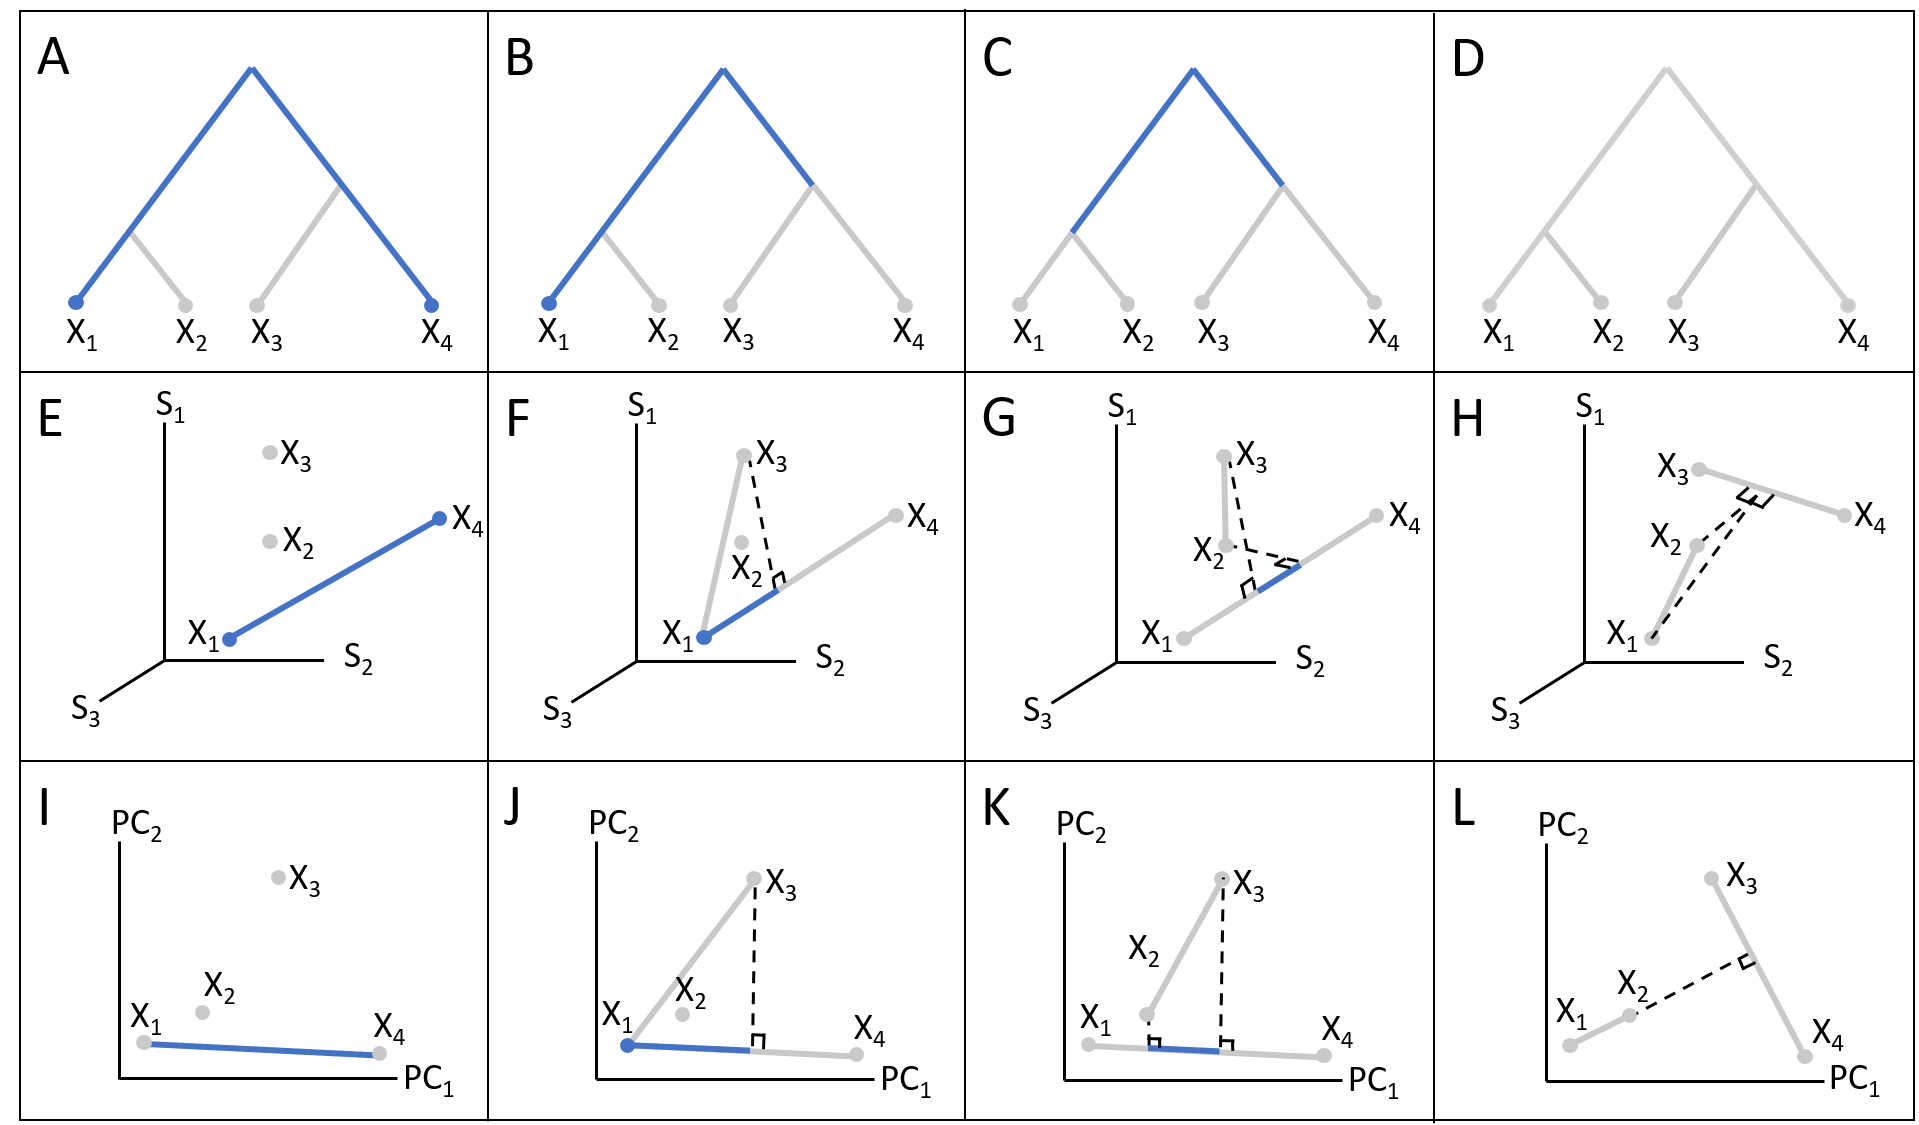
\includegraphics[width=16.5cm]{ppt/schematic_fstats_ppca1.png}
    \centering
    \caption{Schematics showing different interpretations of F-statistics. The columns represent $F_2(X_1,X_4)$, $F_3(X_1;X_3,X_4)$, $F4(X_1,X_3;X_2,X_4)$, $F4(X_1,X_2,X_3,X_4)$. The first row shows a tree interpretation of each statistic, the second row shows F-statistics in an allele-frequency space with three axes representing three SNPs, and the last row is the interpretation of F-statistics on a PCA. Blue lines represent the statistic, and the dotted lines represent orthogonal projections.}
    \label{fig2:overview}
\end{figure}


\subsection{PCA and F-statistics}\label{theory-pca-fstats}

This geometric framework provides an alternate way to understand the properties of F-statistics \cite{oteo-garcia_geometrical_2021}. However, many population genetic studies use a large number of SNPs (in the order of a million), and it is not possible to visualize population vectors in such a high dimensional space. Peter at al. showed that one can do dimensionality reduction on such datasets with PCA, and use the top PCs to estimate F-statistics \cite{peter_geometric_2022}.

We illustrate this in Fig. \ref{fig2:overview}:  $F_2(X_1,X_2)$ can be thought of as the squared Eucledian distance between populations $X_1$ and $X_2$ in PCA-space. Similarly, $F_3(X_1;X_3,X_4)$ is represented as the length of projection of the vector $X_1-X_3$ on $X_1-X_4$. Internal branch length $F_4(X_1,X_3;X_2,X_4)$ can be described as the length of projection of $X_1-X_3$ on $X_2-X_4$ on PCA, and the test of admixture $F_4(X_1,X_2,X_3,X_4)$ is equivalent to the length of projection of $X_1-X_2$ on $X_3-X_4$. We describe a formal relation between PCA and F-statistics (refer to \cite{peter_geometric_2022} for a detailed derivation) in section \ref{theory-pca-fstats}, but here we point out that a joint framework to estimate PCA and F-statistics not only addresses the issue of population assignment in F-statistics, but also can help in interpreting PCA plots \cite{novembre_genes_2008, noauthor_cavalli-sforza_nodate, degiorgio_geographic_2013, francois_principal_2010}. 

Let us assume M populations and S SNPs, such that our dataset $\mathbf{X}$ has the dimension $[M \times S]$, and each entry of $\mathbf{X}$ is an allele frequency $\in$ [0,1]. PCA of mean-centered $\MX$ allows us to project this $[M \times S]$ high dimensional data on a lower dimensional subspace $[M \times q]$. $q = M-1$ represents the case where we retain all the PCs, and thus PCA only rotates X. However, in practice we often only need few PCs (q << M) to explain most variation in the populations \cite{peter_geometric_2022}. A common algorithm to estimate PCs is Singular Value Decomposition (SVD). For this approach we first mean-center $\mathbf{X}$, and then decompose $\mathbf{X}$ into $\mathbf{U}$, $\mathbf{\Sigma}$, and $\mathbf{V^T}$.

$$\mathbf{Y} = \mathbf{C}\mathbf{X} = (\mathbf{U}\mathbf{\Sigma}) \mathbf{V}^T = \mathbf{WL},$$

where $\mathbf{C}$ is the centering matrix such that $\mathbf{C} = \mathbf{I_M} - (1/M)\mathbf{J_M}$. Here $\mathbf{I_M}$ is identity matrix of dimension M, and $\mathbf{J_M}$ is $M\times M$ matrix of all ones. We perform SVD to decompose $\mathbf{Y}$ into a product of $\mathbf{W} = \mathbf{U\Sigma}$ and $\mathbf{L} = \mathbf{V}^T$. In the context of PCA, $\mathbf{W}_{M\times M}$ is a matrix of principal components and contains information about structure, while $\mathbf{L}_{M\times S}$, also known as SNP loadings contains the contribution of each SNP to each PC, and can be used to identify outlier SNPs that may be potential candidates for selection \cite{gower_distance_1966}. 

Since F-statistics can be written as dot products in an allele frequency space (eq. \ref{eq:f_geometric}), and dot products are invariant to rotation, PCA will not change F-statistics as long as we retain all PCs and we can calculate F-statistics from the PCs directly \cite{peter_geometric_2022}:

\begin{align}\label{eq:f_pca}
F_2(X_1,X_4) &= \sum_{s=1}^S(\mathcal{X}_{1s} - \mathcal{X}_{4s})^2\nonumber\\
&= \sum_{s=1}^S(\mathcal{X}_{1s} - \mu_s)(\mathcal{X}_{4s} - \mu_s) = F_2(Y_1,Y_4)\nonumber\\
&= \sum_{q=1}^M(w_{1q} - w_{4q})^2 = F_2(W_1,W_4)\nonumber\\
\end{align}



\subsection{PPCA}\label{theory-ppca}
A difficulty in the practical application of this result is that the geometric considerations of \cite{oteo-garcia_geometrical_2021} and \cite{peter_geometric_2022} only hold for the (generally unobserved) population allele frequencies, but not for sample allele frequencies. In ancient DNA, PCA is most commonly run directly on individual-level genotype data \cite{patterson_population_2006}, and hence on the biased sample allele frequencies. Thus, applying the PCA-based estimator (eq. \ref{eq:f_pca}) to calculate $F$-statistics would likewise result in biased estimate.


Oteo-García et al. resolved this by calculating $F$ statistics using populations with large number of individuals and with no missing dtaa \cite{oteo-garcia_geometrical_2021}. In \cite{peter_geometric_2022}, unbiased estimates of the PCA reconstructions were obtained indirectly by first calculating all pairwise $F_2$-statistics, and then performing a multidimensional-scaling decomposition equivalent to PCA. 

Here, we develop two related approaches that aim to calculate the bias-corrected estimates of $F_2$ from a PCA, by explicitly separating out the error in allele frequencies.

The first approach is based on probabilistic PCA (PPCA) \cite{tipping_probabilistic_nodate, agrawal_scalable_2020}.
PPCA is a dimensionality reduction technique that extends the classical PCA by introducing a probabilistic framework that allows for a homoskedastic error. Like PCA, it is a statistical model that assumes that the observed data is generated from a lower-dimensional latent space, but it adds a constant error term for each observation.

In classical PCA, the goal is to find a linear transformation (rotation) of the data that captures the maximum amount of variance in the original dataset. However, PCA does not provide a probabilistic interpretation of the data and does not explicitly model noise or uncertainty.

PPCA introduces a probabilistic generative model. It assumes that the observed data points are generated by a linear transformation of a lower-dimensional latent space, with an additional Gaussian noise term. The latent variables capture the underlying structure or patterns in the data, while the noise accounts for variability due to sampling error. Setting the Gaussian noise parameter to 0, converges PPCA to PCA.

PPCA models a latent structure of the form $X \sim N(\mathbf{W}Z + \Psi I)$, where X is the observed data, $\mathbf{W}$ is a M x q matrix of linear mappings, $\Psi$ is a Gaussian noise term, $Z$ is a $S$-dimensional latent variable, and $I$ is the identity matrix. Intuitively, $\mathbf{W}Z$ captures the covariance in the observed data, analogous to the F-statistics, and $\Psi I$ is analogous to the bias-correction term.

The goal of PPCA is to estimate the parameters of the model, namely $\mathbf{W}$, $\mu$, and $\Psi$, given the observed data. This is typically done through the standard expectation-maximization (EM) algorithm or maximum likelihood estimation (MLE).

\subsection{LSE}\label{theory-lse}

LSE is a dimensionality reduction technique quite similar to PPCA, with the difference that LSE accounts for the heteroscedasticity in the data \cite{chen_consistent_2015}, and explicitly models the binomial error in genetic data. In this algorithm, we calculate the heterozygosity  $d_{jj} = \frac{1}{S}\sum_i 2x_{ij}(1- x_{ij})$ from $X$. We define $\mathbf{D}$ as a diagonal matrix with $j^{th}$ entry as $\delta_{jj}$. We then estimate covariance matrix $\MG$ = $\frac{1}{S}X^TX - D$. The eigenvectors of $\mathbf{G}$ then span the latent subspace of $\mathbf{L}$ , and the smallest $M-q$ eigenvalues converge to 0 for large M \cite{cabreros_likelihood-free_2019}.


Crucially, if we use \emph{all} the PCs, the $f$-statistics coincide with LSE (see appendix for a derivation): 
\begin{align}
    f_2(X_1, X_4) &= \sum_s (x_{1s} - x_{2s})^2 - d_1 - d_2 \nonumber\\
    &= G_{11} + G_{44} - 2 G_{14}
\end{align}

The covariance used by LSE is an estimated covariance matrix, and its properties differ from the sample covariance matrix used in classical PCA. In particular, sample covariance matrices are positive semi-definite, which means that all eigenvalues are non-negative. In contrast, for an estimated covariance matrix, the expectation of the smallest $M-q$ eigenvalues is zero, and thus an unbiased estimate will have both positive and negative eigenvalues. PCs with negative eigenvalues correspond to imaginary PCs, and thus, we need to adjust eq. \ref{eq:f_pca} as


\begin{align}\label{eq:f_lse}
F_2(X_1,X_4) &= \sum_{q=1}^{M}\mathbb{I}(e_q \geq 0) (w_{1q} - w_{4q})^2 - \sum_{q=1}^M \mathbb{I}(e_q <0) (w_{1q} - w_{4q})^2,
\end{align}
where $e_q$ denotes the $q$-th eigenvalue of $\mathbf{G}$, and $\mathbb{I}$ denotes the indicator function that is 1 when the condition is satisfied, and zero otherwise.


\subsection{Missing data}

\paragraph{$F$-statistics:}
It can be difficult to estimate $F$-statistics when there is high amounts of missing data. A conservative approach to estimate individual-based F-statistics is to only retain sites where data is present from every single individual in the data set. However, even for moderately large data sets that quickly becomes prohibitive: As a toy example, consider a data set with 100 (haploid) individuals with 10\% missing data, and 1,000,000 sites. Out of those, only 26 are expected to be covered in every single individual, which makes this approach not feasible.

Thus, grouping individuals into populations can dramatically increase the number of sites retained. A common practice is to retain sites if at least one individual in each population has data. In the above example, if we grouped the 100 individuals into 10 populations of 10 individuals each, and retained sites where at least one individual in each population carried data, we would expect no missing sites in almost all cases. However, grouping individuals may not be justified when they do not form discrete clusters, or when there are very few samples whose population assignments are unknown.

\paragraph{PCA:}
Missing data is a challenging problem while computing PCA. In this case the issue arises from the inability to perform matrix operations when genotypes are missing. One way to implement a PCA in case of missing data is to start with mean imputation, and then perform PCA to reconstruct the missing values, and keep iterating until convergence \cite{meisner_large-scale_2021}. Another popular way to deal with missing data is to first construct a PCA using samples that have no missing data, and then project the low-coverage samples on this PCA. Projection is a useful way to check if low-coverage samples from the same population fall into the same position as the high coverage ones. Since sampling noise is independent for each sample, projection of samples on a constructed PCA does not require modeling of sampling bias. However, there are certain issues with projection. For example, independent of the quality of projected samples, the position of samples always shifts towards the center of PCA. This phenomenon is called shrinkage, and it occurs due to the loss of the sampling variance. Thus, one needs to use a more complicated method to be able to project samples \cite{smartpca}.

\section{Results}
We evaluate the performance of PCA, PPCA and LSE frameworks and compare to that of admixtools2 \cite{maier_limits_2022} using simulations, and a dataset on Neandertal genetic variation. 

\subsection{Evaluation on simulations}
We simulated 10 populations with 10 individuals each using slendr \cite{petr_slendr_2022}. We use a mutation rate of $10^{-8}$ per base per generation, a recombination rate of $10^{-8}$ per base per generation, and a generation time of 30 years. Fig. \ref{fig2:sim} shows the split times and migration events. 

\begin{figure}[ht!]
    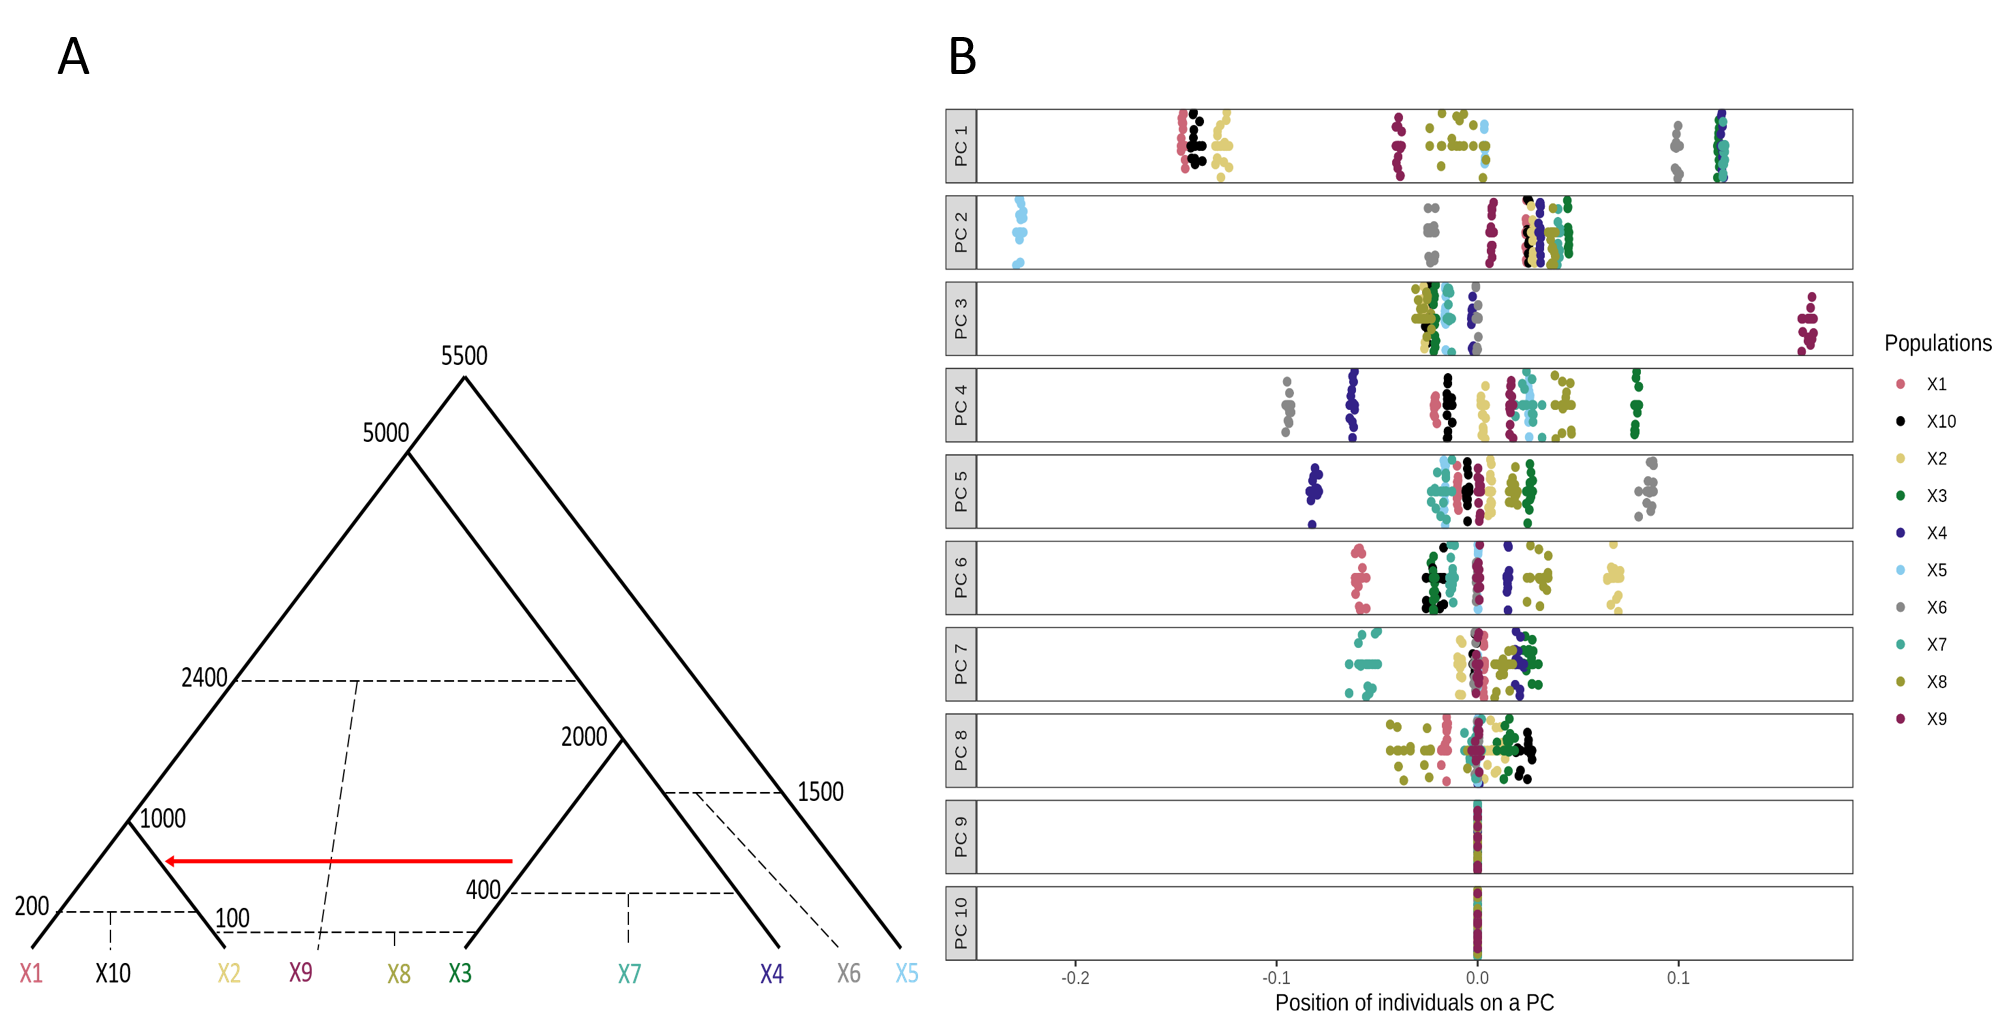
\includegraphics[width=16.5cm]{ppt/sim_all.png}
    \centering
    \caption{Overview of simulated individuals. A. Structure and admixture in the simulated populations represented in the form of a tree. Split time for each node in generations and the admixture branches are shown in dashed lines. The red arrow represents a migration event from $X_3$ to $X_2$. B. PCA of individuals from the simulated individuals in A reflects the population structure represented in the tree.}
    \label{fig2:sim}
\end{figure}

In this simulation, the tree (Fig. \ref{fig2:sim} A) shows the population structure and past admixture events, and the same population structure is reflected by PCs in Fig. \ref{fig2:sim} B. For example, the first PC highlights the internal branch ancestral to X1,X2 and X3,X4. So, X1 and X2 are clustered together (with admixed population X10 in between them), and X3, X4 and X7 form another cluster. X5 is positioned at 0 since it is an outgroup. The second PC highlights the outgroup X5 further. Next, PC 3 shows the axis of variation between X9 and others due to the drift on X9 for many generations. Each PC teases apart a part of the variation in the data. It is interesting to note that a single PC is not informative. One needs to look at all the PCs to get a sense of the population structure. However, the information in the tree and the PC plot is the same, and so the tree can be regenerated from the (top) PCs. 

In this framework, we can then think of F2 as the genetic distance between a pair of populations summing over all PCs. We use eq. \ref{eq:f_pca} to calculate $F_2$ for a pair of populations from the principal components based on either  PCA, PPCA and LSE, and compare F-statistics estimated from these methods to the true theoretical value of the statistic obtained from branch lengths in slendr \cite{petr_slendr_2022}. To demonstrate how we calculate $F_2$ from PCs, Fig. S1 shows the principal components from PPCA for the top 4 PCs plotted in pairs in a conventional manner, and Fig. S2 shows the top variance explained by the top 8 PCs. $F_2(X_1, X_4)$ can then be visualized as the sum of the squared Euclidean distance between $X_1$ and $X_4$ on the top PCs.

We first do a comparison between $f_2$s estimated from PCA, PPCA and LSE with different number of PCs used (Fig. \ref{fig:comparison}). In the top panel of Fig. \ref{fig:comparison}, we use 10 diploid individuals per population, and we see that all three methods are not sensitive to the number of PCs used, as long as enough number of PCs are used (in this case, $\approx 7$). The estimate of $F_2$ based on PCA is only slightly higher than that for PPCA and LSE, as the sampling error term is inversely proportional to the sample size. We next look at a comparison between the three methods using only one individual in each population (Fig. \ref{fig:comparison}). Here we observe that $F2$ estimates from PPCA and LSE are quite close to the true value in all cases, as long as we use at least 7 PCs. and less than 35. However, estimates from PCA get increasingly higher if we add additional PCs. This is expected from theory (section \ref{theory}), since PCA does not account for sampling bias, and, using all PCs, we end up with the biased estimator of $F_2$. Finally, we repeated the estimation of $F_2$s with PPCA and PCA in the presence of $50\%$ missing data (\ref{fig:comparison}C). In this case, PPCA gives reasonably accurate results when the number of PCs used is higher than 7 and lower than around 23, while PCA results are much more noisy. Implementation of LSE is not trivial when there is missingness in data, and is not included in this analysis. 


\begin{figure}[ht!]
    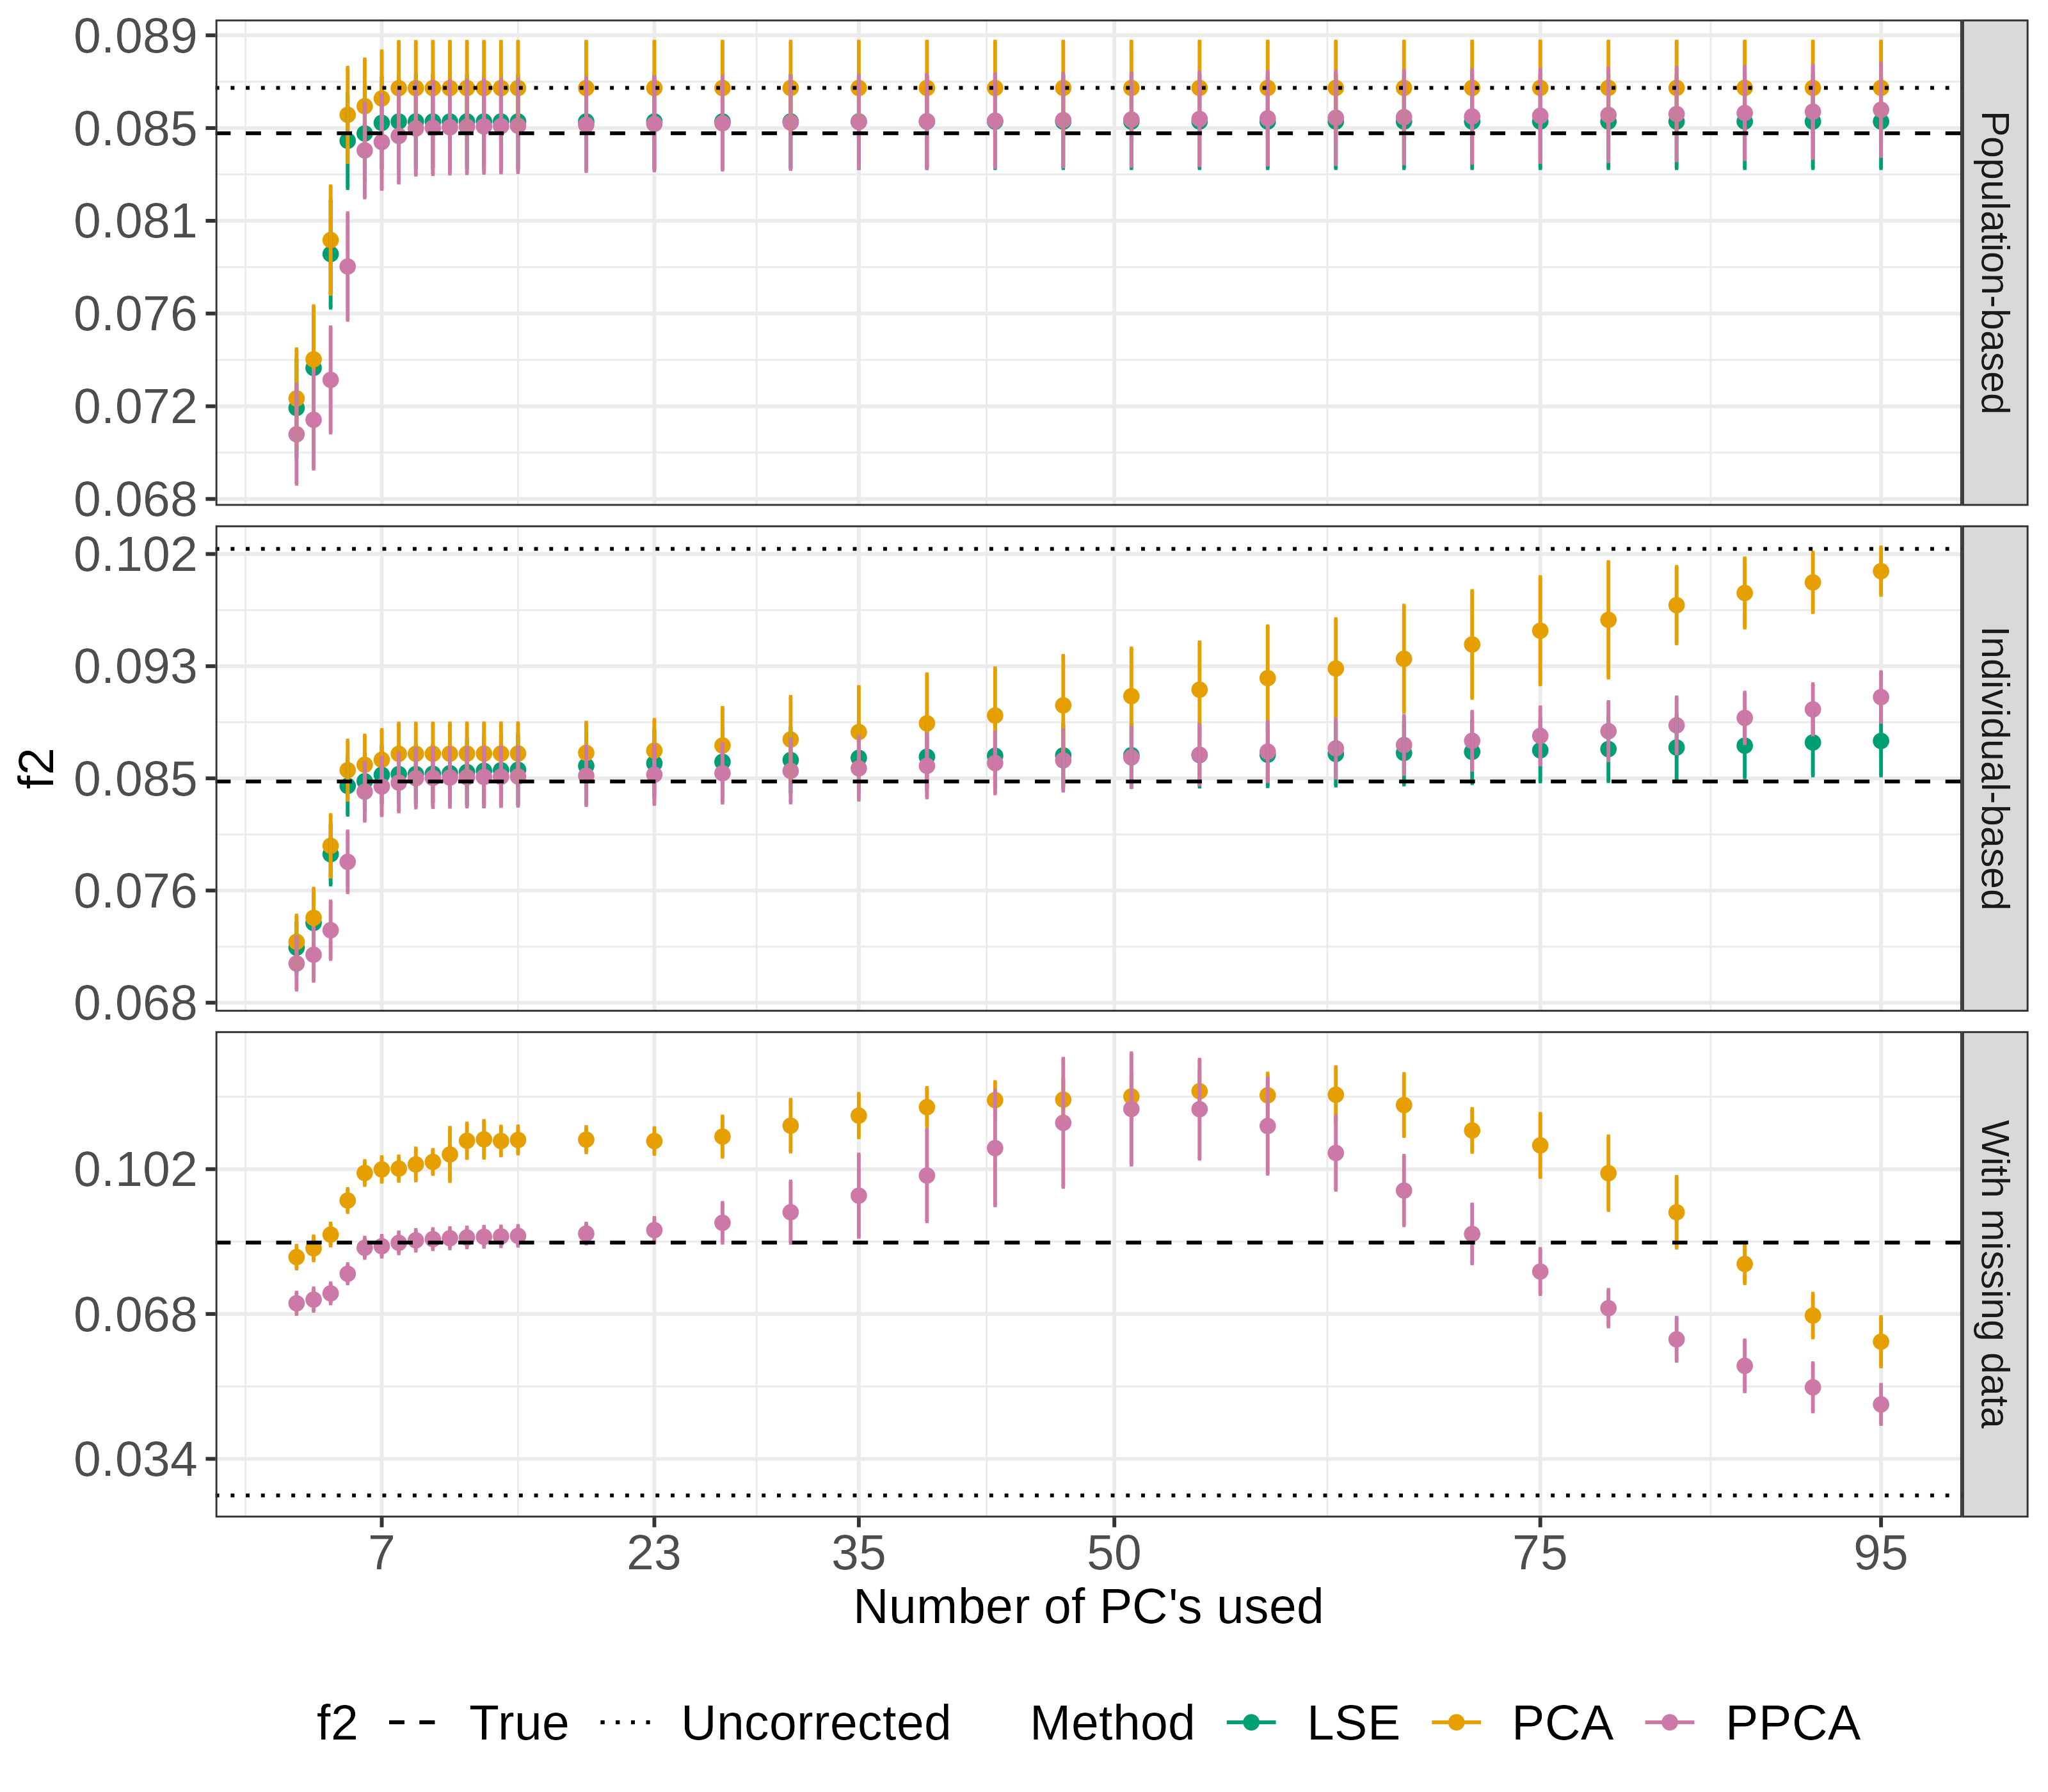
\includegraphics[width=16.5cm]{plots/simfiles_Ne1000_split_times1000/npop10_nind100/missing0.5/mu0.05_main_fig_all_pca.png}
    \centering
    \caption{Comaprison of PCA approaches using $F_2(X_1,X_4)$ estimated using 10 individuals for each population (left), 1 individual for each population (middle), and 1 individual for each population with $50\%$ missing genotypes (right).}
    \label{fig:comparison}
\end{figure}


In the rest of the analyses, we exclude PCA, and compare PPCA and LSE with 8 and 12 PCs to ADMIXTOOLS 2 \cite{maier_limits_2022}, which is a recent re-implementation of ADMIXTOOLS \cite{patterson_ancient_2012} that gives equivalent results. We chose 8 and 12 PCs because the number of PCs to use will not be known in most applications. We first compare $f_2$, $f_3$ and $f_4$ estimated by these methods in an ideal scenario, where each population has 10 individuals, and there is no missing data. In this case we find that the three methods perform well, and get F-statistics close to the truth (fig. S4). 

We next address the issues listed in Introduction section \ref{intro-fstats-estimation}. The first issue is about the estimation of F-statistics when population assignment is difficult, especially when few samples are available. We show that this can be resolved with individual-based F-statistics. In our simulations, we label each individual as a different population, and we sample one individual from each population to calculate F-statistics (fig. S5). We observe that in this case both PPCA and LSE- based frameworks perform atleast as well as ADMIXTOOLS 2 (see table S1) and the mean estimate from each method is close to the true value. However, the error bars for $F_2$ estimates are lower for PPCA compared to ADMIXTOOLS 2, specially for X1 and X2, which have low split-times (standard errors for ADMIXTOOLS 2 estimates for $F_2$ statistics are 0.0018, 0.0015, 0.0027, and 0.0012 while the PPCA-based estimates (scale=8) for the same statistics are 0.0012,0.0012,0.0024 and 0.0011 respectively and for XX LSE). The improved accuracy of PCA-based tools versus ADMIXTOOLS 2 is explained because PCA incorporates a succinct summary of the full data of all the individuals, and thus the PCA-based estimates can ``borrow'' information from related individuals in the sample that are not used to calculate the statistic at hand. In contrast, ADMIXTOOLS 2 has only one individual from each population to assess structure / admixture, and while the estimates based on admixtools 2 are minimum-variance estimators for these subsets of the data \citep{patterson_ancient_2012}, PCA-based methods do better whenever we have data from additional individuals.

\subsection{Missing data}
Next, we address the issue of missing data and evaluate the estimation of these methods when there is random missing data. Our implementation of PPCA on missing data is inspired from EMU \cite{meisner_large-scale_2021}, and is described in Methods section \ref{method-ppca}. We use EMU software for inferring PCs for the calculation of F-statistics. We see that PPCA is not affected by missingness, while ADMIXTOOLS 2 (run with maxmiss=1, so no SNPs are excluded) and EMU results are inflated (Fig. \ref{fig:comparison-adm}, table S1).

\begin{figure}[ht!]
    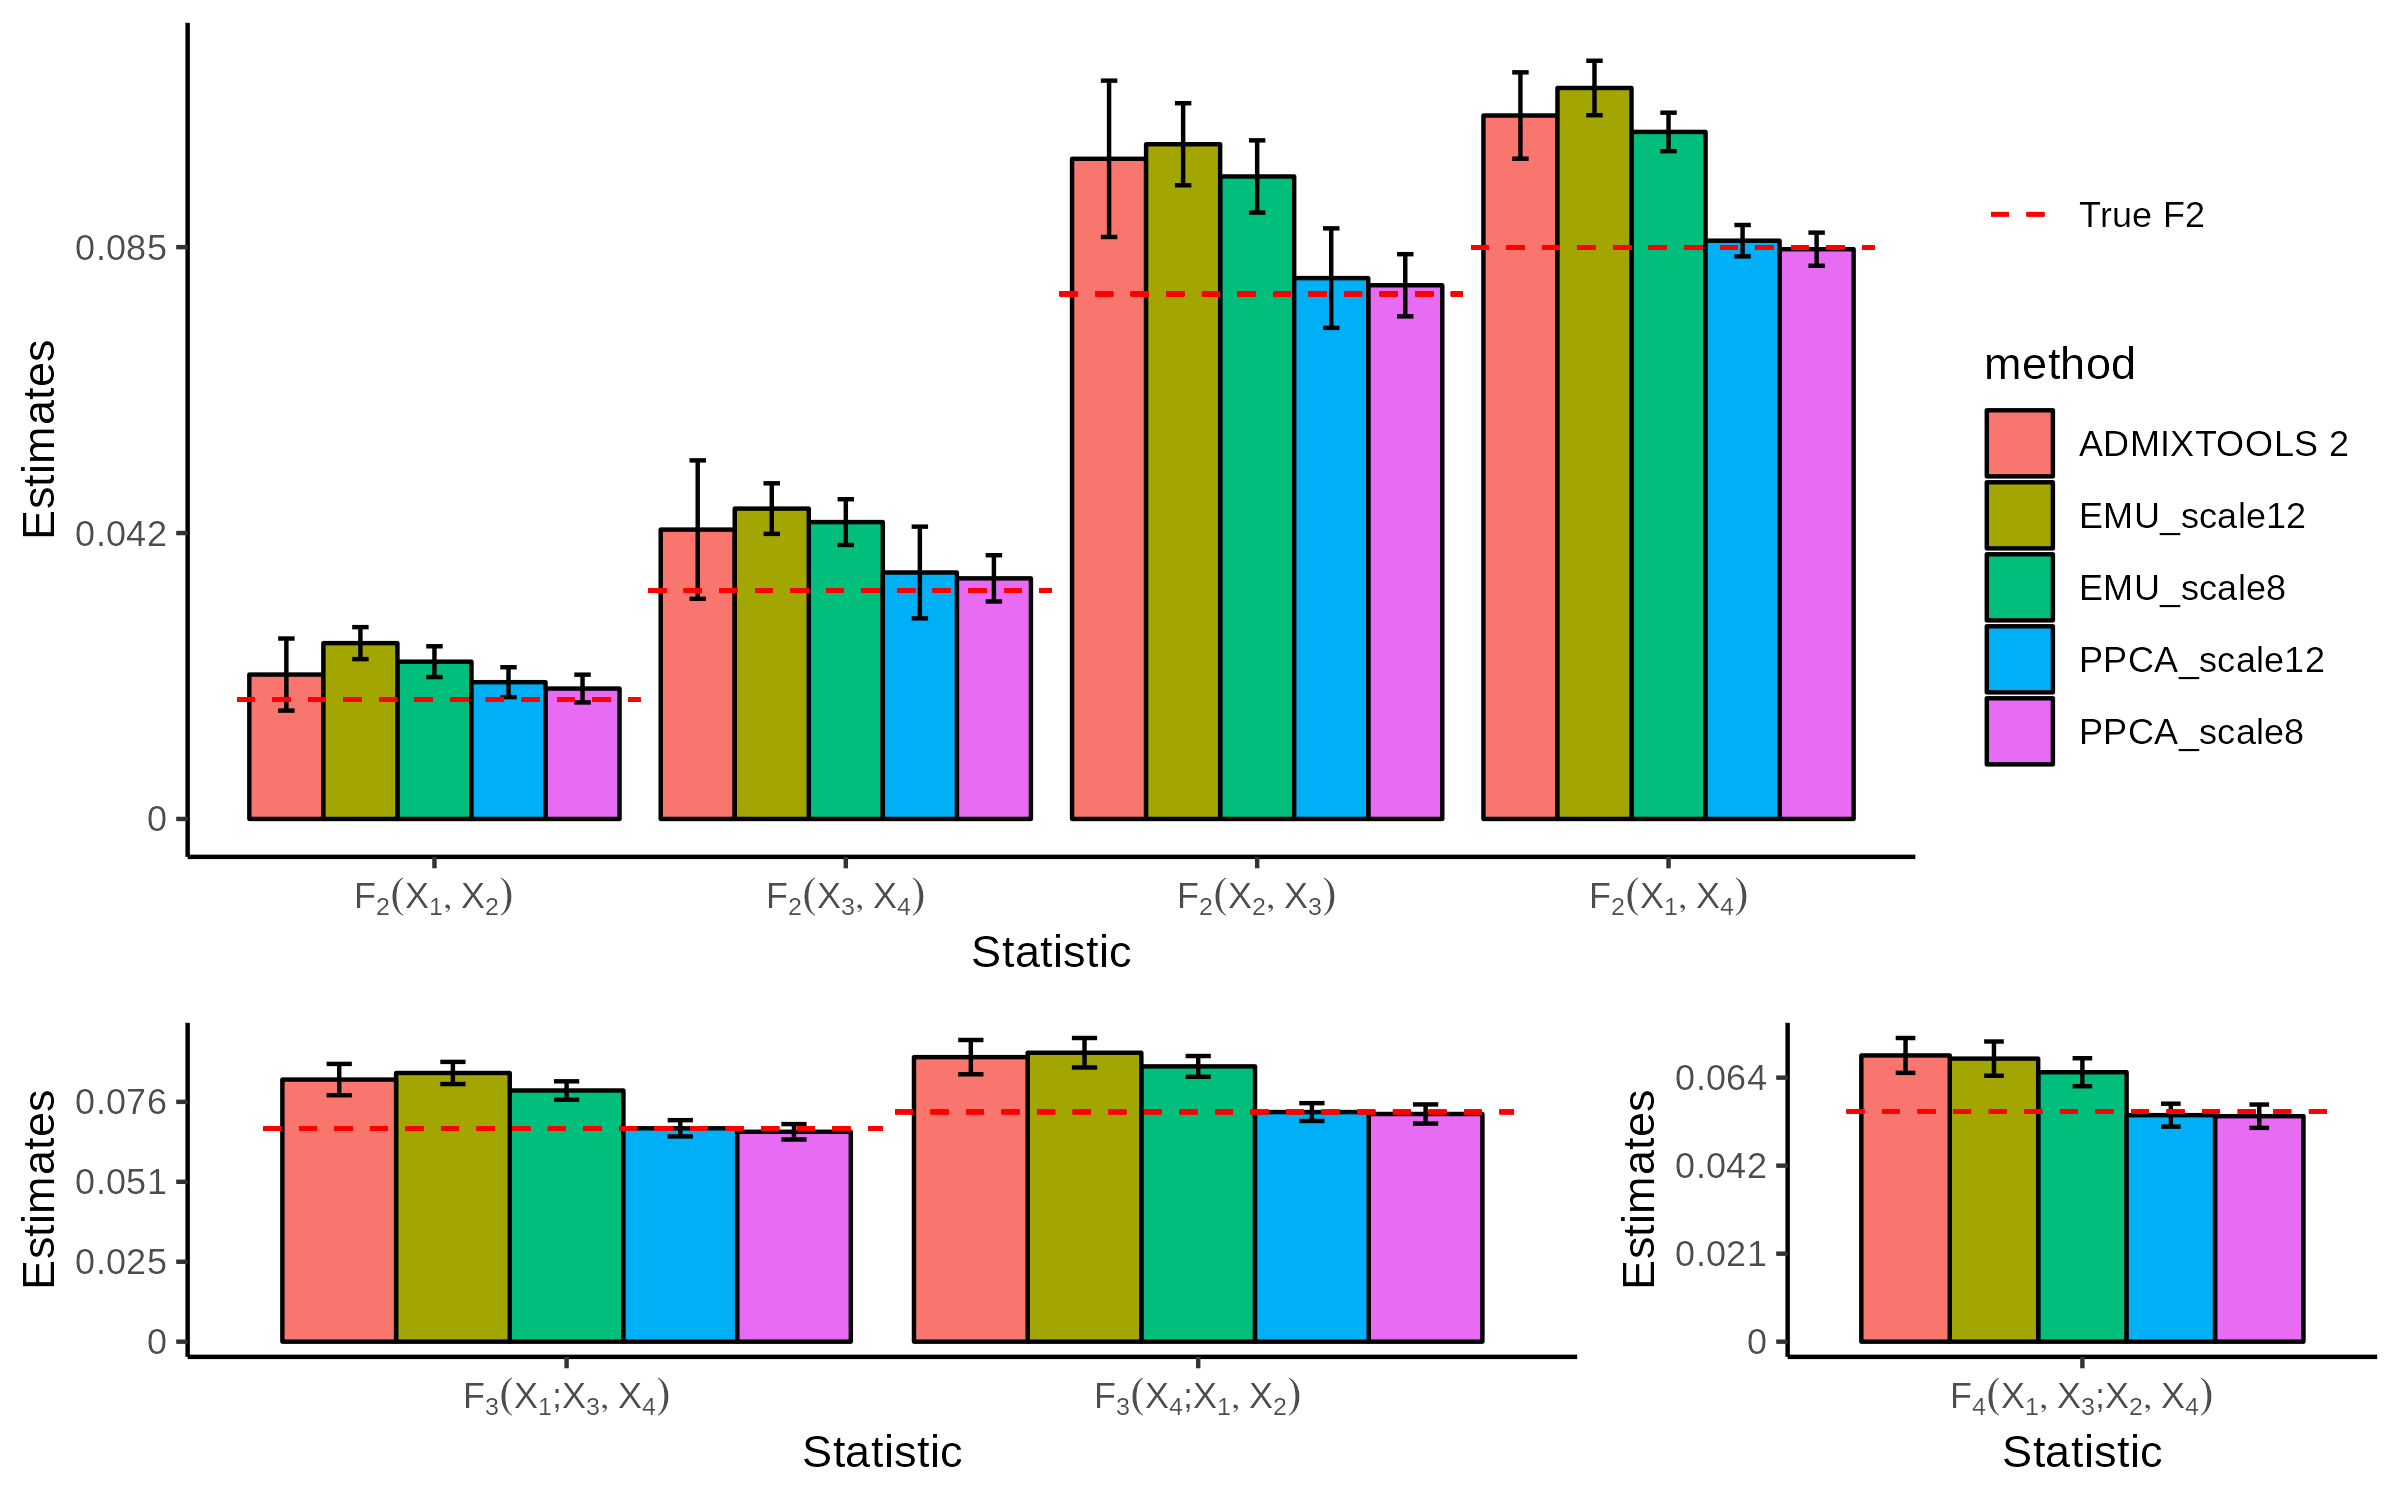
\includegraphics[width=16.5cm]{plots/simfiles/Ne1000/split_times1000/npop10_nind100/missing0.5/plots_8_12/mu0.05_plot_all_1ind_missing.png}
    \centering
    \caption{Comparison of PPCA and PCA to ADMIXTOOLS 2 in the presence of $50\%$ random missingness, using population genotypes from one individual from each population.}
    \label{fig:comparison-adm}
\end{figure}


\subsection{Test of admixture}
A major application of $F$-statistics are tests of admixture \cite{orlando_ancient_2021}. We showed in the previous section that PPCA framework can be used to calculate the point estimates of F-statistics. In this section we show that we can also get standard errors for these estimates using block-jackknife \cite{patterson_modication_nodate}, and use these to do hypothesis testing for admixture. We simulate a gene flow from X3 to X2 500 generations ago with the migration rate of $\mu \epsilon [0, 0.01, 0.05]$. We then compare PPCA framework to ADMIXTOOLS 2. We first test for admixture by checking if the estimate of $F_4(X1,X2,X3,X4)$ is significantly different from 0. We show that when there are 10 individuals in each population, both methods perform well (Fig. S6). In case of 0 migration rate, both methods estimate $F_4$ for all simulations to be close to 0, while at $5\%$ migration rate, ADMIXTOOLS 2 and PPCA-framework have the power to detect admixture (with $F_4$ estimate 2 standard deviations below 0) in $90\%$ and $70\%$ simulations respectively. At migration rate of $1\%$, both the methods are unable to find admixture between $X_2$ and $X_3$, and instead incorrectly predict admixture between $X_1$ and $X_3$ ($F_4$ estimate is 2 standard deviations above the mean) for one simulation. Reducing the number of individuals to 1 from each population reduces the power for both the methods. With $50\%$ missingness, both methods have no false positives in case of 0 migration rate, and at $5\%$ migration rate ADMIXTOOLS 2 and PPCA framework detect admixture in $5\%$ and $35\%$ simulations respectively. At $1\%$ migration rate, ADMIXTOOLS 2 infers admixture between $X_2$ and $X_3$ in 2 simulations and incorrect admixture between $X_1$ and $X_3$ in one simulation, while PPCA framework shows no prediction of admixture.

\begin{figure}[ht!]
    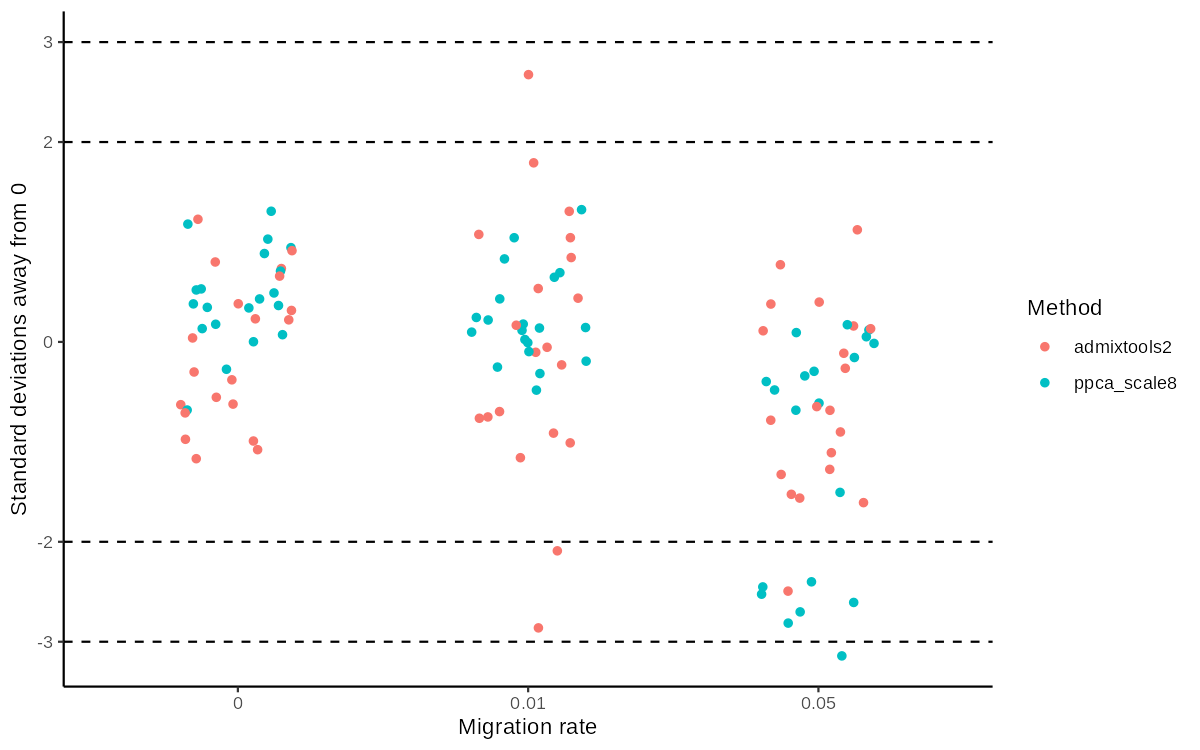
\includegraphics[width=16.5cm]{plots/simfiles/AvgFolder/Ne1000/split_times1000/npop10_nind100/missing0.5/plots_8/hypothesis_test_comparison.png}
    \centering
         \caption{Test for admixture with individual-based $f_4(X_1, X_2, X_3, X_4)$ statistic. We compare ADMIXTOOLS 2 (orange)to PPCA-based-framework (blue) in the presence of 50\% missingness in data.}
    \label{fig:admixture}
\end{figure}

\subsection{Evaluation on neandertal dataset}

To test our framework on real data, we apply it to a published dataset of archaic humans from Eurasia \cite{hajdinjak}. This dataset consists of low-coverage pseudohaploid sequences from late Neandertal specimens from Goyet (Goyet Q56-1), Spy (Spy 94a), Les Cottés (Les Cottes Z4-1514), Vindija (Vindija 87), and Mezmaiskaya caves (Mezmaiskaya1 and Mezmaiskaya2) along with the diploid genotype sequences from high-coverage archaic specimens from Densiova (Altai, Denisova) and Vindija caves (Vindija33.19). We first estimate PCs for this dataset using PPCA, and show that our plot captures all the features of PCA from the authors (Fig. S7, S8). However, we demonstrate that with PPCA, the user can utilize all the specimens to estimate the PCs. 

We analyze how close or distant the low-coverage late Neandertals are to high-coverage Vindija Neandertal using outgroup F3 statistic. F3(Altai, Vindija33.19, X) represents the branch length extending from Altai to the common ancestor of Vindija33.19 and X, where X is a low-coverage late Neandertal. Higher value of F3 denotes closeness of X to Vindija33.19 (Fig. \ref{fig2:overview}). We compare the estimates from PPCA-based framework and ADMIXTOOLS 2, and show that they have a very similar pattern (Fig. \ref{fig:nea_f3}). It is interesting to find that $F_3$(Altai, Vindija33.19, VindijaG1\_L35MQ25) estimated by PPCA framework is higher than that by ADMIXTOOLS 2. We can write $F_3$ as a linear combination of $F_2$'s:


\begin{dmath}
    F_3(Altai, Vindija33.19, Vindija 87) = F_2(Altai, Vindija33.19) + F_2(Altai, Vindija 87) - F_2(Vindija33.19, Vindija 87)\\
\end{dmath}


We looked at the values of the three $f_2$-terms from ADMIXTOOLS 2 and PPCA framework to see why the two methods have different values. We found that $f_2$(Altai, Vindija33.19) and $f_2$(Altai, Vindija 87) have values 0.072 and 0.135 from ADMIXTOOLS 2 respectively. Since both Vindija samples are from the same individual, the $f_3$ values should ideally be the same. PPCA framework outputs the values of $f_2$(Altai, Vindija33.19) and $f_2$(Altai, Vindija 87) as 0.102 and 0.115, which are in line with the expectation. In addition, $f_2$(Vindija33.19, Vindija 87) should ideally be 0. ADMIXTOOLS 2 shows a value of 0.0057, and PPCA-framework gives a value of 0.00094. It is interesting to note that Altai and Vindija33.19 are diploid genomes, and hence $f_2$(Altai, Vindija33.19) estimated with both the methods is similar for the two methods. In contrast, Vindija 87 is a pseudohaploid genome, and in this case we see that PPCA gives expected results and ADMIXTOOLS 2 does not. This is because the unbiased estimator in ADMIXTOOLS 2 for $F_2$ is undefined ($n_{1s}=1$ in eq. \ref{eq:f2_correction}). 

\begin{figure}[ht!]
    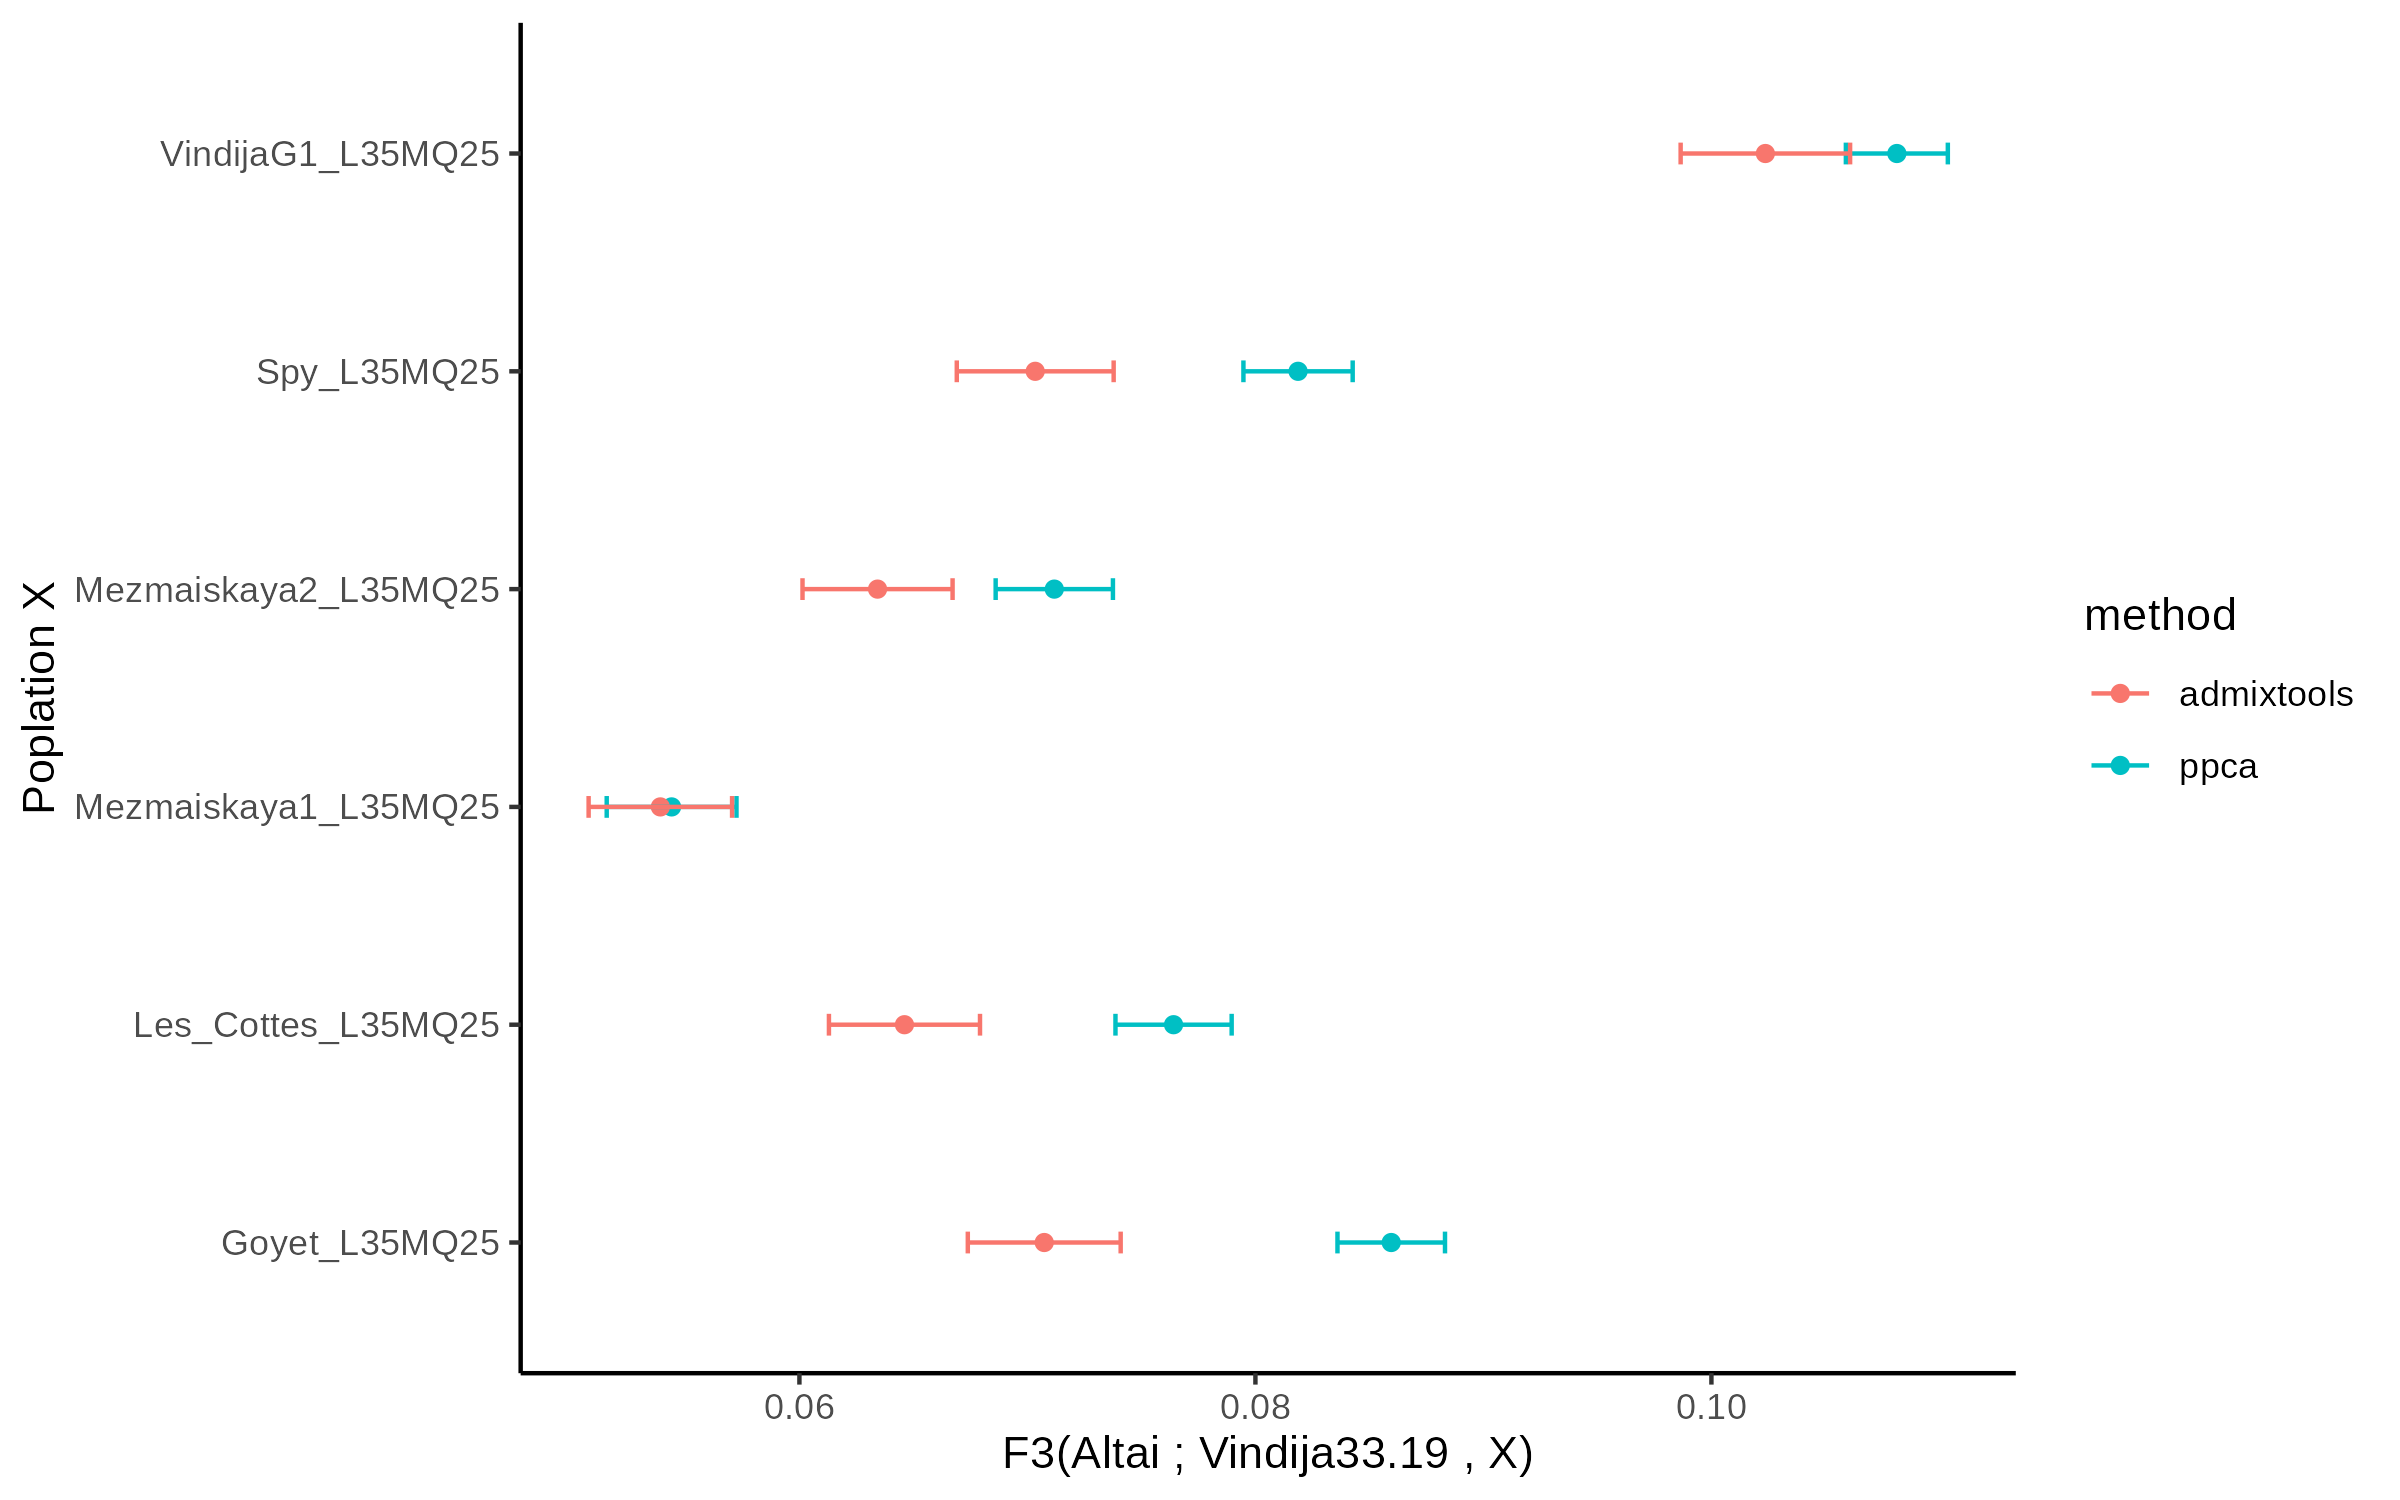
\includegraphics[width=16.5cm]{plots/f3_neandertal.png}
    \centering
    \caption{$F_3$(Altai, Vindija33.19, X) estimated with two methods. Larger value on x-axis represents more proximity to Vindija33.19. Bars show 2 standard errors.}
    \label{fig:nea_f3}
\end{figure}

\section{Methods}

\subsection{PPCA implimentation}\label{method-ppca}

We implement PPCA using maximum-likelihood approach following Tipping and                Bishop \cite{tipping_probabilistic_nodate}, and modify this algorithm to work with missing data. Our approach to handle missingness is inspired from EMU \cite{meisner_large-scale_2021}. We describe our algorithm briefly:
\begin{enumerate}
    \item Mean center data $Y = X - \mu$.
    \item Set missing values to 0.
    \item Perform SVD
    \item Calculate the Gaussian noise parameter $\sigma^2 = \frac{1}{M-q} \sum_{k=M-q}^ M \lambda_k^2$ as the sum of square of the $M-q$ smallest eigenvalues.
    \item Obtain the MLE of the $q^{th}$ eigenvalue as $\lambda_q^2 - \sigma^2$.
    \item Calculate the linear mapping matrix $W = U_q (\lambda_q^2 - \sigma^2I)$.
    \item Reconstruct mean-centered data: $X_R = W(W^TW)^{-1}W^TY$.
    \item Replace missing value with reconstructed values.
    \item Repeat steps 2-7 until convergence.
\end{enumerate}

Our algorithm differs from that of EMU at steps 4-7, which deal with the modelling of the sampling noise and reconstruction of data, and are specific to PPCA algorithm.

\subsection{Calculation of standard errors}

We use a block-jackknife approach to calculate standard errors \cite{maier_limits_2022}. We divide the genome in 2 MB blocks, and estimate PCs and then F-statistics removing a block. Since the statistics obtained are not independent, we calculate variance using this equation \cite{maier_limits_2022}:

\begin{align}\label{eq:bjk_var}
V &= \frac{1}{g} \sum_{i=1}^g \frac{s_i}{S-s_i} (\hat{\theta} - \theta_i)^2
\end{align}

Here, V is the variance of a statistic $\theta$, g is the number of blocks, s is the number of sites in block i, and S is the total number of sites.


\section{Discussion}
In this study, we present a statistical framework to jointly compute PCA and $F$-statistics. Many ancient genetic studies use both of these tools, but use slightly different assumptions, slightly different models and different software for them. In contrast, our joint framework allow us to make sure that assumptions are consistent throughout the analysis. The key advantage is that the effect of modelling assumptions become apparent, and this also allows us to make novel recommendations about how PCA-based analyses should be performed and interpreted.

The connections between $F$-statistics and PCA allow us to provide a better understanding on how different PCA algorithms emphasize different parts of the data, and how they emphasize population structure versus sampling noise.

In particular, $F$-statistics enable quantitative interpretation of PCA-plots, where distances on a PCA are directly proportional to genetic differentiation, and orthogonal projections can directly be used to test for admixture. 


\paragraph{Classical PCA}
Classical PCA is mathematically the simplest, and still the most widely used method for visualizing population structure. It has an interpretation in terms of pairwise coalescent times \citep{mcvean_genealogical_2009}. However, because classical PCA incorporates \emph{all} variation in the data, it does not distinguish between variation due to population structure, and variation due to sampling. This can lead to problems: For example, one cannot directly project additional samples to a PCA, instead some correction is required  otherwise some ``shrinkage'' occurs where new samples are projected closer to the origin \citep{patterson_population_2006}.  Thus,  in our opinion classical PCA should be the primary choice for analyzes primarily aimed at quality control, because incorporating noise allows it to reveal technical artifacts and outliers Effects of different sequencing or capturing techniques, will very often be visible on a PCA-plot, while they may be more hidden and only partially corrected in PPCA.

\paragraph{Probabilistic PCA}. Our results suggest that the methods that seperate sampling noise from population structure, such as PPCA AND LSE, are preferable to classical PCA when the primary goal is to depict population structure. PPCA is the simpler of the two methods, because it assumes homoskedastic noise, i.e. that all samples have the same heterozygosity / sampling variance. As \cite{tipping_probabilistic_nodate} showed, without missing data, the maximum-likelihood estimator of PPCA results in virtually identical PCA plots compared to those obtained from a classical PCA; the only differences are that the axes for the first few PCs will be rescaled, and that the majority of PCs are set to zero. (see Fig. S2 and Fig S3).


\paragraph{LSE}
LSE goes one step further by adding heteroskedastic, binomial noise. This ensures that both PCA and $F$-statistics use the exact same modelling assumptions, and thus LSE-based PCA plots are directly comparable to $F$-statistics. This relationship is exact if all PCs are used. However, one advantage of LSE is that the eigenvalues corresponding to the PCs irrelevant for population variation have an expectation of zero. Since these eigenvalues are directly proportional to the amount of variance explained per PC, and to the contribution of these $F$-statistics, we expect that truncating them will yield good results, which is indeed what we see in our simulations (Fig. S4). 

In real data, this expectation of zero for the eigenvalues will typically yield both positive and negative eigenvalues, which is why the equation for computing $f_2$ needs to be adjusted (eq. \ref{eq:f_lse}), and subtract the contribution to $F_2$ by PCs that have negative eigenvalues. Alternatively, we could interpret these PCs as being on the imaginary axis on the complex plain, but both interpretations are simply a result from the fact that we design an unbiased estimator for a quantity with an expectation of zero. 

From a theoretical point of view, the model optimized in LSE is more desirable to that in PPCA, because it takes into account that different individuals might have different heterozygosities. However, the advantage of PPCA is that it works relatively well with missing data, and even for single pseudohaploid samples, which are common in ancient DNA applications (Figure 5). 


\paragraph{Projection PCA}. A further approach that is used for ancient DNA is to project data low-coverage data onto a ``reference''-data set. This has three useful advantages: First, the overall shape of the PCA only depends on the reference data set. Thus, PCA-plots using the same reference data become directly comparable, which can be useful as a quick way of assessing population variation, e.g. using the Western Eurasian PCA used in studies of Holocene ancient DNA studies from Europe and Western Asia \citep{haak_massive_2015}. Second, it deals with missing data in the projected samples, because often only a subset of sites are required for an accurate projection. Third, it also deals with sampling noise in the projected sample, because the sampling noise is orthogonal to the variation in the reference data set, and thus gets removed by the projection.

However, the drawback of using projections, and why they, in our opinion, are inferior to probabilistic PCA, is that they do not capture the full variation in the data. In particular, only the variation in the reference data is considered, but not the variation that is private to the projected samples. 

In terms of $F$-statistics \cite{peter_geometric_2022}, 

\begin{equation*}
    F_2(X_1, X_2) = \underbrace{F_2^{\text{(PCA)}}(X_1, X_2)}_{\text{visible in projection PCA}} + \underbrace{F_2^{\text{(Projection)}}(X_1, X_2)}_{\text{hidden in projection PCA}}
\end{equation*}

This is particularly problematic when projecting ancient human samples onto a modern reference data set, because the differentiation between ancient human population is often considerably larger than that between present-day populations \citep{haak_massive_2015, lazaridis_ancient_2014}, and thus projection PCA have no quantitative interpretation.


\subsection{Plotting PCs}
One of the major benefits of using $F$-statistics and PCA in a joint framework is that it enables a quantitative interpretation of PCA. Thus, our results directly suggest some recommendations for how PCs should be plotted when displaying population genetic variation is desired. 

First, the scale at which PCs are plotted matters, and the units on the different PCs are comparable (Figure \ref{fig2:sim}B). Thus, we recommend that PCA-biplots should be plotted with ``fixed'' aspect ratios where the x- and y-axes have the same units and scale, contrary to the current common practice where the axes are scaled arbitrarily (e.g. \cite{novembre_genes_2008, peter_genetic_2020}). It also highlights the benefits of plotting PCs on a shared axis  such as in Figure \ref{fig2:sim}B, where the decreased variance explained by each subsequent PC is directly visualized, and tens of PCs can be plotted jointly.

Second, it has been a ``best-practices'' suggestion that PCs are plotted along the proportion of variance explained by each PC (e.g. ). While we think this holds, it is important to recognize that different PCA algorithms handle this differently: In classical PCA, the proportion of variance is out of the total variance, including population structure, within-population variation and sampling noise. In contrast, in PPCA the number of PCs retained is a parameter, which \emph{sets} the proportion of variance explained by population structure. Thus, we obtain the (user-controlled) proportion of variance due to noise (corresponding to $\Psi$), and the proportion of variance each PC explains as a proportion of the variation explained by population structure. 

This latter interpretation is identical to that obtained through LSE, where the number of PCs retained is not fixed. Thus, the percent of variation explained between classical PCA, PPCA and LSE are not directly comparable.

\subsection{Grouping individuals}
A benefit of the interpretation that we developed is that it demonstrates when and how we can use PCA to group individuals into  populations for $F$-statistics-based analysis. 
Thus, the groupings of individuals into populations becomes a result of the analysis, as opposed to an \textit{a priori} assumption set by the researcher.

This \textit{a priori} grouping may lead to difficulties in analyses, for example when dealing with recent migrants, or when grouping sparsely sampled populations. As ancient genetic sampling becomes more dense, recent migrants have become increasingly prevalent in data sets. These migrants are important, because they allow us tracking of movements -- often over large distances -- within the last handful of generations. Thus, these recent migrants have become an important focus of study and it is desirable to distinguish recent migration from the more distant-in-time migration that is ordinarily the focus of $F$-statistic analyses.

A PCA will reveal such recent migrants as outliers that group with their population-of-origin, whereas they would be missed by $F$-statistics.

In sparsely sampled populations, it is often necessary to group individuals that span relatively large areas or times to get to a usable sample size, particularly for regions where DNA preservation is poor. However, grouping genetically distinct individuals can be risky, as population substructure can invalidate the interpretation of $F$-statistic-tests \cite{peter_admixture_2016}. However, PCA provides a meaningful and simple way to assure that populations are devoid of relevant substructure: If individuals  cluster tightly on \emph{all} PCs that are meaningful for between-cluster variation, they can safely be grouped. However, if there is within-population variation that is correlated with other populations, then $F$-statistic-tests cannot be used to test for admixture. 

As discussed above, these considerations hold particularly when using a PCA method that separates sampling noise from population structure, such PPCA or LSE. For classical PCA, clustering will also be impacted by sample quality and depth - which can be separated out effectively by the probabilistic methods.


\paragraph{Dealing with missing data}
We show that ADMIXTOOLS 2 estimates of individual-based $F$-statistics are inflated when there is $50\%$ missing sites in the data, while PPCA-based algorithm is not affected.
It is interesting to note that an inflation of $F$-statistics has not been reported in literature, and we find that in presence of multiple individuals in each population, and few missing sites, the default setting of the software filters out all the sites with missing data, and the $F$-statistics are not affected. In this study, to compare PCA-based methods to ADMIXTOOLS 2, we used the option to use all sites regardless of the amount of missingness. Hence, our results suggest that while the estimates of ADMIXTOOLS 2 with default settings are unbiased in case of missing data, the option to use sites with missing data (maxmiss) should be used with caution.

\paragraph{How many PCs should be used?}
Our framework is able to deal with missing data illuminate us to point out that the conventional method to estimate F-statistics suffers from two major problems. First, one needs to assign individuals to discrete populations which may not be justified for humans, and is difficult to do with ancient samples. And second, the estimates are inaccurate in presence of high amounts of missing genotypes, another characteristic of ancient DNA. We present a PCA-based framework to estimate F-statistics while taking in account these issues. We compare the statistics estimated with different PCA approaches, and show that all approaches work well on ideal simulations with enough samples. In case of individual-based F-statistics, both PPCA and LSE outperform classical PCA, and we provide a PPCA algorithm for the case of missing data. We compare PPCA framework to ADMIXTOOLS 2, and find that our framework outperforms ADMIXTOOLS 2 to estimate individual-based F-statistics with missing data.

PCA is widely used in population genetics to visualize clusters of individuals that may represent populations, and clines potentially representing historical admixture. Moreover PCA may reveal fine-scale structure in the population \cite{waldman_genome-wide_2022}. PCA's ability to condense complex genetic data into interpretable dimensions enhances our understanding of human evolution, migration, and admixture events, and throws light on the intricate mosaic of our species' history. However the visualization results from PCA may be influenced by the choice of PCs used, normalization, and the choice of populations used. \cite{elhaik_principal_2022}. We provide a way of quantifying the results of a PCA with F-statistics so that all PCA's can be comparable and can use the same normalizations. Such a quantification using all the top PCs also makes it more straight-forward to justify a visual result made with 2 PCs.

We used a PPCA-based framework with the Neandertal data to estimate PCs utilizing all the samples. This approach is more straight-forward than authors' approach to first estimate the PCs using high-coverage genomes, and then project the low-coverage genomes. We show that we can accurately estimate outgroup $F_3$ statistic from the PCs. We find that $F_2$ calculated using diploid genotype data with our framework is comparable to that of ADMIXTOOLS 2. However, ADMIXTOOLS 2 can not be used to estimate $F_2$ with pseudohaploid data since the unbiased estimator in ADMIXTOOLS 2 is undefined in this case. We show that our framework provides accurate estimates even with pseudohaploid samples. 

One limitation of this framework is the need to perform multiple PPCAs to obtain standard errors, which can be computationally expensive. Further studies are needed to design a statistical framework that can estimate the errors using SNP loadings, and therefore can work fast with large datasets.

To summarize, we present a method to perform PCA and F-statistics jointly and show that this approach not only improves estimates of F-statistics, but also provides a solution to the standardization and quantification of PCA. Our framework is available on github as a snakemake pipeline: https://github.com/DivyaratanPopli/A-joint-framework-for-PCA-and-F-statistics.





\section{Appendix}

We provide the procedure to estimate LSE as laid out by \cite{cabreros_likelihood-free_2019}. We define a symmetric matrix $\hat{\mathbf{H}}$:
\begin{equation}
    \hat{\mathbf{H}} = \frac{1}{S}\mathbf{X}^T\mathbf{X} - \hat{\mathbf{D}},
\end{equation}

Here, $X$ is the (uncentered) genotype matrix with shape $m \times S$ , $\hat{\mathbf{D}}$ is a matrix of diagonal entries ``correcting'' heterozygosities and $S$ is the number of SNPs.

In particular $d_{ij} = 0 $ for $i \neq j$ and, 
\begin{equation}
    d_{ii} = \frac{1}{S}\sum_{k=1}^S x_{ik}(2-x_{ik}),
\end{equation}
for diploid data. The correction term given by \cite{reich_reconstructing_2009} and \cite{patterson_ancient_2012} is different by a factor of 4:
\begin{equation*}
    d_{ii}' = \frac{1}{S}\sum_{k=1}^S \frac{x_{ik}}{2}(1-\frac{x_{ik}}{2}) = \frac{d_{ii}}{4}
\end{equation*}

The factor of 4 is due to the use of allele frequencies instead of genotypes, i.e. their approach would estimate $\hat{\mathbf{H}}$ (again for diploid data)
\begin{equation*}
    \hat{\mathbf{H}'} = \frac{1}{S}\frac{\mathbf{X}^T}{2}\frac{\mathbf{X}}{2} - \frac{\hat{\mathbf{D'}}}{4} = \frac{\hat{\mathbf{H}}}{4},
\end{equation*}
and so the parametrizations are equivalent, but will differ by a factor of four.

Thus, 
\begin{subequations}\begin{align}
    h_{ii} &= \frac{1}{S}\sum_{k=1}^S x_{ik}^2 - d_i \\
    h_{ij} &= \frac{1}{S}\sum_{k=1}^S x_{ik}x_{jk} 
\end{align}\end{subequations}
Consider now
\begin{align}
    f_{ij} &= h_{ii} + h_{jj} - 2 h_{ij}\nonumber\\
     &= \frac{1}{S}\sum_{k=1}^S x_{ik}^2 - d_i + \frac{1}{S}\sum_{k=1}^S x_{jk}^2 - d_j - \frac{2}{S}\sum_{k=1}^S x_{ik}x_{jk}\nonumber \\
    &= \frac{1}{S} \sum_{k=1}^m (x_{ik} - x_{jk})^2 - d_i - d_j \\
    &= F_2(i,j)\nonumber
\end{align}

Hence the matrix $\hat{\mathbf{H}}$ can be used to estimate unbiased $F_2$-statistics.



\section{removed stuff}

\section{appendix old}
\begin{equation}
    \hat{\mathbf{H}} = \frac{1}{m}\mathbf{X}^T\mathbf{X} - \hat{\mathbf{D}},
\end{equation}

Here, $\MX$ is the (uncentered) genotype matrix and $\hat{\mathbf{D}}$ is a matrix of diagonal entries ``correcting'' heterozygosities and $m$ is the number of SNPs.

In particular $d_{ij} = 0 $ for $i \neq j$ and, 
\begin{equation}
    d_{ii} = d_i = \frac{1}{m}\sum_{k=1}^m x_{ik}(2-x_{ik}),
\end{equation}
for diploid data. The correction term given by Reich 2009 and Patterson 2012 is different by a factor of four:
\begin{equation*}
    d_{ii}' = \frac{1}{m}\sum_{k=1}^m \frac{x_{ik}(2-x_{ik})}{4} = \frac{d_{ii}}{4}
\end{equation*}.
The difference is explained that they use allele frequencies instead of genotypes, i.e. their approach would use (again for diploid data)
\begin{equation*}
    \hat{\mathbf{H}'} = \frac{1}{m}\frac{\mathbf{X}^T}{2}\frac{\mathbf{X}}{2} - \frac{\hat{\mathbf{D'}}}{4} = \frac{\hat{\mathbf{H}}}{4},
\end{equation*}
and so the parametrizations are equivalent, but will differ by a factor of four.

Thus, (TODO: double-check if rows/columns are aligned, sum should be over SNP)

\begin{subequations}\begin{align}
    h_{ii} &= \frac{1}{m}\sum_{k=1}^m x_{ik}^2 - d_i \\
    h_{ij} &= \frac{1}{m}\sum_{k=1}^m x_{ik}x_{jk} 
\end{align}\end{subequations}
Consider now
\begin{align}
    f_{ij} &= h_{ii} + h_{jj} - 2 h_{ij}\nonumber\\
     &= \frac{1}{m}\sum_{k=1}^m x_{ik}^2 - d_i + \frac{1}{m}\sum_{k=1}^m x_{jk}^2 - d_j - \frac{2}{m}\sum_{k=1}^m x_{ik}x_{jk}\nonumber \\
    &= \frac{1}{m} \sum_{k=1}^m (x_{ik} - x_{jk})^2 - d_i - d_j \\
    &= F_2(i,j)\nonumber
\end{align}

Hence the matrix $\hat{\mathbf{H}}$ can be used to estimate $F_2$-statistics (possibly instead of PPCA?).



We describe two issues in accurate estimation of population allele frequencies:

1. Humans may not fit into well-differentiated discrete populations, except in cases where the populations have been isolated due to geographical features \cite{novembre_genes_2008}. The estimation of population allele frequencies depends on the assignment of individuals to discrete populations, and may be affected by miss-assignment especially when few samples are available. 

2. Missing data in some individuals for certain sites can make it difficult to get accurate allele frequency estimates at those sites. One commonly used solution to this problem is to filter out all the sites with missing data. However, this may make the number of sites available for F-statistics quite small. E.g., for 100 individuals with $10\%$ randomly missing sites, the available number of sites after filtering out positions with missing data would be $\approx26$ out of a total 1,000,000 sites. 

Studies using PCA generally use specific PCs to visualize population structure or admixture, and the choice of the PCs used can be quite subjective \cite{elhaik_principal_2022}. Estimation of F-statistics from PCA quantifies, using all the important PCs, what the researcher has visualized using seemingly arbitrary PCs.

However, a limitation with such a framework is that it is possible to define F-statistics in terms of PCs only when allele frequencies are known, and need not be estimated. This is due to the fact that PCA does not filter the noise in the data due to sampling. In addition, missing data can affect the computation of PCs, and subsequently F-statistics.


We would point out here that in ancient DNA studies PCA is sometimes used as quality-control step by constructing PCs using high-quality samples, and projecting the low-quality samples which may be from the same populations or even the same individuals as the high coverage samples. In the presence of contamination from present-day people, reference bias, ascertainment bias or batch effects, the projected sample may not overlap with an identical high-coverage sample. These biases and issues are not resolved with PPCA/LSE either, since PPCA only models sampling noise. 


\subsection{F-statistics with PPCA/LSE}
In this study, we develop a statistical framework to estimate F-statistics between individuals in a PPCA framework. We show that PPCA explicitly models the error due to the sampling bias in allele frequencies. In addition, we demonstrate that PPCA based framework is not sensitive to random missing data, and so it can be used to visualize individuals in PCA-space without having to project lower quality samples.

We explain that PPCA provides a natural framework to estimate F-statistics with small sample-size and missing data. We show formal hypothesis tests for admixture and compare our results to admixtools2 \cite{maier_limits_2022} on simulations. Finally we show the use of this framework on published datasets from neolithic Haak et al. and upper Paleolithic humans (Mateja). 

Mathematically, the PPCA model can be represented as follows \cite{tipping_probabilistic_nodate}:

Latent variable model:
Latent variables: $Z \sim N(0, I)$, where Z is a S-dimensional latent variable, and I is the identity matrix.

Latent-to-observed mapping: $X = WZ + \mu + \Psi$, where X is the observed data, W is a M x q matrix of linear mappings, $\mu$ is the mean of the observed data, and $\Psi$ is a Gaussian noise term.

Prior distributions:

Prior on the latent variables: $P(Z) = N(0, I)$

Prior on the noise term: $P(\Psi) = N(0, \sigma^2I)$, where $\sigma^2$ is the variance of the noise.

Likelihood function:
$p(X|Z, W, \mu, \Psi) = N(X|WZ + \mu, \sigma^2I)$

\section{old stuff}
\subsection{PCA}

One way to estimate F-statistics 

the estimation of allele frequencies can also be affected by large amounts of missing data. Since F-statistics are dependent on the ascertainment scheme, random missing data reduces the number of overlapping sites greatly.
PCA is a powerful method to visualize population structure but it can be difficult to interpret \citep{cavalli-sforza1993, novembre_stephens_2008, degiorgio_rosenberg2013}. In particular, the population structure in PCA is a function of expected pairwise coalescence times \citep{mcvean_genealogical_2009}, and thus is not explicitly tied to a particular scenario; different histories may yield similar or identical PCAs. 

Thus, parameter estimation, model comparisions and formal tests of admixture are usually not carried out in PCA. 

(add section here introducing the general idea of PCA, explain how it deals with error/noise  and difference between probabilistic and regular PCA. Possibly also explain how people use PCA as a QC-step to detect batch effects, and how that compares with PCA used for population structure (i.e. Ainash' question from your talk))

F-statistics are a useful tool to quantify population structure, and provide tests for admixture. Hence, a common pipeline in many population genetic studies is to analyze PCA plots to look for visible patterns that could be due to past admixtures, followed by formal test with F-statistics \cite{lazaridis_ancient_2014,lazaridis_genomic_2016}. F-statistics use population allele frequencies to test for admixture, and hence the accuracy of these tests is limited by the accuracy of allele frequency estimates \cite{peter_admixture_2016}. Whereas F-statistics estimates are robust when there are enough high quality samples, we show that low number of samples and missing data decrease the accuracy of these tests.

A major issue when working with ancient DNA is low number of individuals and missing data. This issue is exacerbated due to difficulty in assigning some of the individuals to discrete populations. Especially in the case of humans samples, we know that the genetic samples do not strictly belong to discrete populations, but form a continuous spectrum in the allele frequency space \cite{oteo-garcia_geometrical_2021}. Hence, it is a step in the right direction to think of a method to estimate F-statistics in a structure-aware framework. The easiest way to think about this is using PCA. PCA does not require assignment of individuals to discrete populations, and it has been shown that F-statistics can be estimated conveniently from distance between populations on PCA space \cite{peter_geometric_2022}. However, PCA distances are inaccurate when population sizes are small since PCA does not explicitly model sampling bias in the allele frequencies (see section XX). In addition, PCA is sensitive to missing data, and this makes it difficult to work with ancient DNA. 



In this study, we develop a statistical framework to estimate F-statistics between many populations in a probabilistic PCA framework.  that probabilistic PCA (PPCA) explicitly models the error due to the sampling bias in allele frequencies. In addition. we demonstrate that PPCA based framework is not sensitive to random missing data, and so it can be used to visualize individuals in PCA-space without having to project lower quality samples.

Finally, we show that PPCA provides a natural framework to estimate F-statistics with small sample-size and missing data. We show formal hypothesis tests for admixture and compare our results to admixtools2 cite{admixtools paper} on simulations. Finally we show the use of this framework on published datasets from neolithic Haak et al. and upper Paleolithic humans (Mateja). 





\section{older stuff}
There are several tools available to understand genetic diversity, and can be classified as the tools that make minimal assumptions to summarize population structure, and the tools that infer demographic parameters. Former set of tools includes f-statistics \cite{patterson_ancient_2012}, PCA \cite{mcvean_geneaylab=""logical_2009}, MDS \cite{wang_comparison_2009}, Structure \cite{pritchard}, Admixture  
- There are different tools to study diversity: 1) tools that make minimum assumptions like fstatistics, PCA, MDS, Structure, Admixture, 2) tools that can be used to infer demographic parameters.
- Many studies use PCA followed by f-statistics in their pipline. Peter et al., show that these analyses reveal the same biological signal, and can be done jointly.
- This framework has limitation: population allele frequencies are not known.
- Here we present an approach based on pPCA, and show that it is a more natural framework since it can take in account the errors associated with allele frequency estimation.

\subsection{Theory}
- f-statistics, and the sampling error terms in f2.
- PCA and relation to f-statstics.
- pPCA/PCA1 (Waaij et. al.) as a framework for dimentionality reduction taking in account the sampling error.

\subsection{results}
- Advantage in estimating PCs: Fig.1: PCA plot with standard errors

- Advantage in estimating f-statistics: We compare f-statistics from pPCA, PCA1, PCA, admixtools2 in terms of accuracy (and speed?). Fig.2: point estimates of f2's for slendr simulations where we have both ancient and modern populations. Fig.3: Examples of f4 test of treeness with different cases of migrations, we can also show a case of f3 test of admixture.

- Application to a published dataset (Fig.4)

\subsection{Discussion}
- One key advantage of this framework is that both point estimates and standard errors for PCA and fstatistics are estimated together in a consistent way.
- This is a step towards solving the issue with the assumption of discrete populations.
- This would be quite useful for cases where assigning individuals to populations can be difficult.
- Future work: 1) A faster way of estimating standard errors. 1) to get uncertainty from snp loading. 2) Hypothesis testing 

- This approach could also help with missingness as shown by Meisner et al. 
- pPCA makes it easy to analyse modern and ancient data together without having to project samples.

\subsection{Methods}
- Simulation method and parameters used


\section{Abstract}

Studies of genetic variation now routinely include data from thousands of individuals representing complex historical and temporal structure. Understanding and modeling patterns of genetic variation between large numbers of individuals and populations is thus a key challenge in the usage of genetic data to answer questions about evolutionary history. 
Principle Component Analysis (PCA) and F-statistics sensu Patterson are both widely used for this purpose, but are usually analyzed dis-jointly. Here, we present a new framework based on 
probabilistic PCA to jointly estimate principal component and F-statistics from large panels of data. A key advantage of our approach is that we can calculate individual-based F-statistics efficiently, and so population assignments become a result rather than an a priori assumption. Furthermore, probabilistic PCA provides a natural framework for incorporating missing data, a common issue in ancient DNA analyses. Taken together, our results greatly simplify the analysis of large population genetic data sets, and allow for fast data exploration and statistical testing in a unified and consistent framework.

\section{Background}

\subsection{Why study genetic diversity}
The genetic diversity of human populations has been shaped by historical and environmental factors over hundreds of thousands of years. Therefore, a key objective of population genetics is to analyze the observable variations and patterns in order to understand and reconstruct the demographic and evolutionary history of our species. 

\subsection{The general pipeline}

A general pipeline consists of a method to summarize the data with minimal assumptions. Examples are PCA, MDS, Structure, Admixture. These methods show a qualitative picture, but do not estimate a biologically meaningful parameter. And so, it is difficult to design statistical tests for the results of such methods. However, such qualitative results are generally followed by quantifiable methods based on f-statistics. F-statistics with 2,3, or 4 populations assumes a null-model as a tree-like structure and a deviation from the tree-like structure is represented the alternate model.

\subsection{PCA and fstatistics}
PCA is a method to rotate the dataset in a way that so that the axes that are analysed and plotted are aligned with the dimensions explaining the highest variation in the data. This is a way to do dimensionality reduction, and provides a way to do better data visualization. Ben[2020] showed that PCA and f-statistics are related, and   


\section{Introduction}
\subsection{Why combine pPCA and F-statistics?}

\paragraph{In case of no missing data}

- Calculating f-statistics between populations already assumes clustering of individuals into populations. PCA shows this clustering, but it would be useful to quantify the distance between individuals to filter for individuals that cluster, spot outliers, and identify substructures.

-Faster calculation of f-statistics, when only few PCs are used. Calculation of pPCA may take some time, but afterwards f-statistics is less time taking. And since people anyway do both PCA and f-statistics, overall this would reduce time.

-admixture proportions from f-statistics using pca. We can check if it's more reliable.
\paragraph{In case of missing data}

- In case of admixturegraphs, missing data may reduce total snps (although, missing sites would be less if allele frequencies are calculated from available individuals in populations). pPCA may help in cases with e.g., few ancient individuals from each population with a lot of missing data. 

- In case of ancient DNA, may help to include libraries with missing data instead of projecting them?
\newpage
\section{Practical application ideas}
This is a list of ideas we could pursue. Goal would be to pick a few that would be easiest to accomplish.
\begin{enumerate}
    \item Evaluate whether we use PPCA to calculate individual-based $F$-statistics accurately and fast?
    \begin{enumerate}
        \item in presence of missing data
        \item for multivariate analyses including qpadm/qpgraph
        \item include samples projected onto PCA
    \end{enumerate}
    \item Grouping individuals in populations
    
    \item Can we get confidence intervals on PCA?
        \begin{enumerate}
            \item Resampling SNPs
            \item Resampling individuals
            \item Calculate uncertainty based on SNP loadings
            \begin{enumerate}
                \item For SVD $\mathbf{X} = \mathbf{(UD)V}^T = \mathbf{PV}^T$, we might be able to use the correlation in the entries of $\mathbf{V}$ to estimate the ``effective'' number of SNPs
            \end{enumerate}
        \end{enumerate}
    \item Practical programming
        \begin{enumerate}
            \item Write software tool that jointly computes individidual-based F-stats and PCA
        \end{enumerate}
    \item Data analysis -- find a good data set or scenario to analyze
        \begin{enumerate}
            \item Standard Western Eurasian PCA
            \item Indian data
            \item Some application that Stephan / Wolfgang are working on
        \end{enumerate}
    \item Looking at qpadm/qpwave
        \begin{enumerate}
            \item qpadm projects samples into a subspace made from a subset of samples. As these samples are not orthogonal, this subspace is likely highly non-orthogonal and therefore tricky to work with. Doing PCA before doing qpadm could be helpful. 
        \end{enumerate}        
\end{enumerate}


\section{Projecting onto prob PCA}

For PCA, we can write $X_{[n \times p]} = USV^T$ and the PCs are given by $SV^T$. , and we would project by


\begin{align}
    X &= USV^T \\
    U^T X &= SV^T \\
    XVS^{-1} &= USV^TVS^{-1} \\
    &= U \\
    U^T Y &= Y_{proj}\\
    XVS^{-1}Y &= Y_{proj}
\end{align}
and we can project using $U^TY $ for new data $Y$. 


\newpage
\section{F-tests using Wishart-log-likelihoods}
Consider the $F_4$-statistic
\begin{align}
    F_4(A-B, C-D)&= Cov(A-B, C-D)\\ &= Cov(A, C) + Cov(B,D) - Cov(A,D) - Cov(B,D)\\
\end{align}


\subsection{PCA to Covariance matrix}
If we have a matrix of PCs, $\BP$, then $\mathbf{Y} = \BP\BP^T$ is an estimate of the covariance matrix. Consider the random variables $(A-B)$ and $(C-D)$. If we assume they are jointly normally distributed, then their joint distribution will again be normally distributed with mean zero and covariance matrix 
\begin{equation}
    \bf{X} = \begin{pmatrix} 
    y_{11} + y_{22} - 2 y_{12} & y_{13} + y_{24} - y_{14} - y_{23} \\
    y_{13} + y_{24} - y_{14} - y_{23} & y_{33} + y_{44} - 2 y_{34} &  \\
    \end{pmatrix}
\end{equation}
where the $y$ are the entries of the  covariance matrix obtained from the PCA. Practically, we can either first calculate $Y$ (if we want all $F$-stats), or first subset $\BP$ to the four pops involved.

The off-diagonal elements of $\MX$ are precisely the $F$-statistics we aim to calculate. And thus we set up a test to see whether they are zero.


\subsection{Derivation of the test statistic}
The sampling distribution of a covariance follows a Wishart distribution. This is a $p \times p$ - matrix-valued probability distribution that is parametrized by a degree-of-freedom parameter $n$ and a covariance matrix $\MS$, also of dimension $p \times p$. The simplest way to generate Wishart random variates is, 
\begin{equation}
    \MX = \sum_{i=1}^n Y_i Y_i^T
\end{equation}
where $Y_i \sim N(0, \MS)$. We also have 
\begin{align}
    E[\MX] &= n\MS \\
    mode(\MX) &= (n-p-1) \MS
\end{align}

The log-likelihood of a Wishart Distribution is

\begin{align}
    \log P(\MX | \MS, n) &= -\frac{np}{2} \log(2) -  \frac{n}{2}\log\left|\MS\right| - \Gamma_p\left(\frac {n}{2}\right ) + \frac{n-p-1}{2} \left|\MX\right| -\frac{1}{2}\operatorname{tr}({\MS}^{-1}\MX)\\
    &\propto  -\frac{n}2\log\left|\MS\right|   -\frac{1}{2}\operatorname{tr}({\MS}^{-1}\MX)\nonumber\\
    %&= -\frac{n}2 \log \left( \sigma_{11}\sigma_{22} - \sigma_{12}^2\right) - \frac{1}{2}\frac{\sigma_{22}x_{11} - 2\sigma_{12}x_{12} + \sigma_{11}x_{22}} {\sigma_{11}\sigma_{22} -  \sigma_{12}^2} 
    &= -\frac{n}2 \log \left( \sigma_{11}\sigma_{22} - \sigma_{12}^2\right) - \frac{1}{2}\frac{\sigma_{22}x_{11} + \sigma_{11}x_{22} -2 \sigma_{12}x_{12}} {\sigma_{11}\sigma_{22} -  \sigma_{12}^2} 
\end{align}
where the last step assumes a $2\times 2$ matrix. 
Under H0, we have $\sigma_{12} = 0$, therefore
\begin{align}
    \log P(\MX | \MS_0, n) &= -\frac{n}2 \log \left( \sigma_{11}\sigma_{22}\right) - \frac{1}{2}\left[\frac{x_{11}}{\sigma_{11}}  + \frac{x_{22}}{\sigma_{22}}\right] 
\end{align}
This likelihood is easily separatable and we can estimate $\sigma_{11}$ from $x_{11}$ and $\sigma_{22}$ from $x_{22}$ directly.

The log-likelihood-ratio statistic can then be calculated as 

\begin{align}
    R &= - 2 \log  \left( \frac{P(\MX | \MS_0, n)}{ P(\MX | \MS, n)} \right)  \nonumber\\
    &=2 [\log P(\MX | \MS, n) - \log P(\MX | \MS_0, n) ] \nonumber\\
    &=  n \log \left( \sigma_{11}\sigma_{22}\right) - n \log \left( \sigma_{11}\sigma_{22} - \sigma_{12}^2\right)  \nonumber\\
    &+  n\left[\frac{x_{11}}{\sigma_{11}}  + \frac{x_{22}}{\sigma_{22}}\right] 
    - n\frac{\sigma_{22}x_{11} + \sigma_{11}x_{22} -2 \sigma_{12}x_{12}} {\sigma_{11}\sigma_{22} -  \sigma_{12}^2} 
\end{align}
using the estimates $\sigma_{ij} = \frac{x_{ij}}{n}$ we get
\begin{align}
    R&\approx n \log \left( x_{11}x_{22}\right) - n \log \left( x_{11}x_{22} - x_{12}^2\right) + 2n - 2n  \nonumber\\
     &= n  \log \left( \frac{x_{11}x_{22}}{x_{11}x_{22} - x_{12}^2}  \right)
\end{align}
 A $\log(n^2)$ term in each of the log-terms cancels. The statistic $R$ is asymptotically $\chi^2$ distributed with one degree of freedom.

If we instead use the mode $\sigma_{ij} \approx \frac{x_{ij}}{n-3}$:

\begin{align}
    R&\approx n  \log \left( \frac{x_{11}x_{22}}{x_{11}x_{22} - x_{12}^2}  \right)
+2 (n-3) \frac{x_{11}x_{22} - x_{12}^2} {x_{11}x_{22} -  x_{12}^2} 
    - 2(n-3) \nonumber\\
     &= n  \log \left( \frac{x_{11}x_{22}}{x_{11}x_{22} - x_{12}^2}  \right)
\end{align}

\subsection{Comparison to Cavalli-Sforza \& Piazza, 1975}
The authors propose 
\begin{equation}
    R = \frac{|\MX|}{|\MS|}
\end{equation}
where $|\cdot|$ is the determinant. For $2 \times 2$ matrices,


\begin{align}
|\MX| &= x_{11}x_{22} - x_{12}^2 \\
|\MS| &= x_{11}x_{22} \\
    R &= \frac{ x_{11}x_{22} - x_{12}^2}{ x_{11}x_{22}} =1 - \frac{ x_{12}^2}{ x_{11}x_{22}}\\
    T &= -2 n \log (R) = 2 n \log \left( \frac{ x_{11}x_{22}}{ x_{11}x_{22} - x_{12}^2}\right)
\end{align}

The factor of 2 might be wrong..

\subsection{other statistics}
for $x_{12}$  small, we may further approximate
\begin{align}
         R &= n  \log \left( \frac{x_{11}x_{22}}{x_{11}x_{22} - x_{12}^2}  \right)\nonumber\\
            &= n  \log ( x_{11}x_{22}) - n\log ({x_{11}x_{22} - x_{12}^2} )\nonumber\\
            &= n  \log ( x_{11}x_{22}) - n\log \left[x_{11}x_{22} \left(1  - \frac{x_{12}^2}{x_{11}x_{22}} \right)\right]\nonumber\\
           &=n  \log \left( 1 - \frac{x_{12}^2}{x_{11}x_{22}}  \right) \nonumber\\
           &\approx  n \frac{x_{12}^2}{x_{11}x_{22}} 
\end{align}
This is the coefficient of determination, which is the square of the correlation coefficient
\begin{equation}
    r =  \sqrt{R/n} = \frac{x_{12}}{\sqrt{x_{11}x_{22}}}
\end{equation}

for which we have a $t$-distributed null
\begin{equation}
    r \sqrt{\frac{n-2}{1-r^2}} \sim t(n)
\end{equation}
The Fisher-Transform then yields
\begin{equation}
    \frac{1}{2} \log\left(\frac{1+r}{1-r}\right) = \arctan(r) \sim N(0,1)
\end{equation}
which simplifies to 
\begin{equation}
    \arctan(r) = \frac{1}{2} \log\left(\frac{\sqrt{x_{11}x_{22}} + x_{12}}{\sqrt{x_{11}x_{22}} - x_{12}}\right) 
\end{equation}
This statistic is normally distributed under the null-hypothesis.


in tests with a simple bivariate normal, all of them behaved equally well.


\newpage
\section{Calibrating the standard errors of $F$-stats}
Traditionally, the standard errors of F-stats are estimated using a block-Jackknife approach. However, the block size is usually hard to estimate, and may impact the resulting values.

\subsection{What do the standard errors measure?}
There are two types of uncertainty:
\begin{itemize}
    \item \textbf{sampling uncertainty}, that stems from the fact that we only have a small sample from each population. Because it depends on the sample, we expect these uncertainties to be independent for each sampled population
    \item \textbf{evolutionary uncertainty} there is also uncertainty due to the randomness in evolution. In particular, the realized mean allele frequencies in populations will be different from those expected under some model. 
\end{itemize}

\subsection{Covariance of $F_2$-statistics}
\begin{align}
    K &= Cov( (X_1- X_2)^2, (X_3 - X_4)^2 )  \nonumber\\
    &= Cov(X_1^2, X_3^2) + Cov(X_1^2, X_4^2) + Cov(X_2^2, X_3^2) + Cov(X_2^2, X_4^2) \nonumber\\
    &- 2\left [ Cov(X_1^2, X_3X_4) + Cov(X_2^2, X_3X_4) + Cov(X_3^2, X_1X_2) + Cov(X_4^2, X_1X_2)) \right]\nonumber\\
    &+ 4\left[ Cov(X_1X_2, X_3X_4)\right]\nonumber\\
\end{align}
At the same time, we have

\begin{align}
    F_4^2 &=  Cov(X_1 - X_2, X_3 - X_4) ^2 \nonumber\\
    &= \big[ Cov(X_1, X_3) + Cov(X_2, X_4) - Cov(X_1, X_4) - Cov(X_2, X_3)   \big]^2\nonumber\\
    &= Cov(X_1, X_3)^2 + Cov(X_2, X_4)^2 + Cov(X_1, X_4)^2 + Cov(X_2, X_3)^2  \nonumber\\
    &+2 \big[ Cov(X_1, X_3) Cov(X_2, X_4) + Cov(X_1, X_4) Cov(X_2, X_3)\big] \nonumber\\
    &-2 \big[ Cov(X_1, X_3) Cov(X_1, X_4) + Cov(X_1, X_3) Cov(X_2, X_3)\big] \nonumber\\
    &-2 \big[ Cov(X_2, X_4) Cov(X_1, X_4) + Cov(X_2, X_4) Cov(X_2, X_3)\big] \\
    &= (E[X_1^2] + E[X_2^2])(E[X_3^2] + E[X_4^2]) \nonumber\\
    &+2 \big[ E[X_1X_3]E[X_2X_4] + E[X_1 X_4] E[X_2 X_3]\big] \nonumber\\
    &-2 \big[ E[X_1 X_3] E[X_1 X_4] + E[X_1 X_3] E[X_2 X_3]\big] \nonumber\\
    &-2 \big[ EX_2 X_4] E[X_2 X_3] + E[X_2 X_4] E[X_2 X_3]\big] \\
    &= (E[X_1^2] + E[X_2^2])(E[X_3^2] + E[X_4^2]) \nonumber\\
    &+2 \big[ E[X_1X_3]  [ E[X_2X_4] - E[X_1 X_4]] +  E[X_2 X_3] [ E[X_1 X_4]  - E[X_1 X_3] ]\big] \nonumber\\
    &-2 \big[ EX_2 X_4] E[X_2 X_3] + E[X_2 X_4] E[X_2 X_3]\big] \nonumber\\
\end{align}
But we have $Cov(A,B) = E[ (A-E[A])(B-E[B])] = E[AB] - E[A]E[B]$ and 
\begin{align}
Cov(A, B)Cov(C, D) &= E[ (A-E[A]) (B-E[B])] E[(C-E[C])(D-E[D])]\nonumber\\
&= E[AB]E[CD] =  E[ABCD] - Cov(AB, CD)
\end{align}

\newpage
\section{Notes on PCA1 of van Waaij et al}
van Waaij et al. suggest at PCA on a matrix of the following form for PCA
\url{https://doi.org/10.48550/arXiv.2302.04596} (their PCA1). This approach is further motivated by eq 7 in \url{https://www.ncbi.nlm.nih.gov/pmc/articles/PMC6707457/}, which is a very technical (but probably useful) reference.

\begin{equation}
    \hat{\mathbf{H}} = \frac{1}{m}\mathbf{X}^T\mathbf{X} - \hat{\mathbf{D}},
\end{equation}
where $\MX$ is the (uncentered) genotype matrix and $\hat{\mathbf{D}}$ is a matrix of diagonal entries ``correcting'' heterozygosities and $m$ is the number of SNPs.

In particular $d_{ij} = 0 $ for $i \neq j$ and, 
\begin{equation}
    d_{ii} = d_i = \frac{1}{m}\sum_{k=1}^m x_{ik}(2-x_{ik}),
\end{equation}
for diploid data. The correction term given by Reich 2009 and Patterson 2012 is different by a factor of four:
\begin{equation*}
    d_{ii}' = \frac{1}{m}\sum_{k=1}^m \frac{x_{ik}(2-x_{ik})}{4} = \frac{d_{ii}}{4}
\end{equation*}.
The difference is explained that they use allele frequencies instead of genotypes, i.e. their approach would use (again for diploid data)
\begin{equation*}
    \hat{\mathbf{H}'} = \frac{1}{m}\frac{\mathbf{X}^T}{2}\frac{\mathbf{X}}{2} - \frac{\hat{\mathbf{D'}}}{4} = \frac{\hat{\mathbf{H}}}{4},
\end{equation*}
and so the parametrizations are equivalent, but will differ by a factor of four.

Thus, (TODO: double-check if rows/columns are aligned, sum should be over SNP)

\begin{subequations}\begin{align}
    h_{ii} &= \frac{1}{m}\sum_{k=1}^m x_{ik}^2 - d_i \\
    h_{ij} &= \frac{1}{m}\sum_{k=1}^m x_{ik}x_{jk} 
\end{align}\end{subequations}
Consider now
\begin{align}
    f_{ij} &= h_{ii} + h_{jj} - 2 h_{ij}\nonumber\\
     &= \frac{1}{m}\sum_{k=1}^m x_{ik}^2 - d_i + \frac{1}{m}\sum_{k=1}^m x_{jk}^2 - d_j - \frac{2}{m}\sum_{k=1}^m x_{ik}x_{jk}\nonumber \\
    &= \frac{1}{m} \sum_{k=1}^m (x_{ik} - x_{jk})^2 - d_i - d_j \\
    &= F_2(i,j)\nonumber
\end{align}

Hence the matrix $\hat{\mathbf{H}}$ can be used to estimate $F_2$-statistics (possibly instead of PPCA?).
The detailed justification of this can be found in \href{https://stats.stackexchange.com/questions/14002/whats-the-difference-between-principal-component-analysis-and-multidimensional}{this statsexchange post  that will need to be adapted}.

Thus, this might be a useful alternative to PPCA to calculate $F$-statistics:

\begin{enumerate}
    \item Calculate $\hat{\mathbf{H}} = \frac{1}{m}\mathbf{X}^T\mathbf{X} - \hat{\mathbf{D}}$
    \item Double-Center $\hat{\mathbf{H}}$: $\mathbf{H}_c = \mathbf{C}\hat{\mathbf{H}}\mathbf{C}$, where $\mathbf{C}$ is a centering matrix
    \item Obtain PCs using an eigendecomposition of $\mathbf{H}_c$: $\MP\MP^T = \mathbf{H}_c$
    \item Calculate $F_2$ from the smaller space $\MP$
\end{enumerate}

\section{Standard errors and effective number of SNPs}
An issue in calculating standard errors for $F$-statistics is that SNP are usually correlated, and so standard variance and standard error calculations will fail.

let us assume $n$ populations can be represented by some population structure model that is parameterized by some covariance matrix $\MX$. We do not observe SNPs, but rather we have a noisy sample $\MG_{[S \times n]}$ at $S$ loci.

Let, as above, denote the data matrix as $\MG$, which is a noisy version of an allele frequency matrix $\MX$, and we assume we can do a PCA on some estimate of $\hat{\MX}$ as 
$\ML\MZ = \hat{\MX}$ where $\ML$ are the orthonormal SNP-loadings and $\MZ$ are the PCs. For example, we could do that using probabilistic PCA or the Cabreros-Storey-PCA

We are interested in statistics of the form 
\begin{equation}
    F_{ij} = (X_i - X_j)^2
\end{equation}
which can be estimated from $\MG$ using the unbiased estimator of Patterson et al.
\begin{equation}
    f_{ij} = \frac{1}{S}\sum_{s=1}^n (g_{si} - g_{sj})^2 - H_i - H_j.
\end{equation}

alternatively, we can also obtain an estimate from the decomposition of  $\hat{\MX}$ as
\begin{equation}
    p_{ij} = \frac{1}{S}\sum_{p=1}^n (z_{si} - z_{sj})^2,
\end{equation}
this sum is over PCs. This estimator has thus the advantage that it can be computed a lot faster since typically $n \ll S$, and if $X$ is low-rank we can even truncate the sum

An issue is the calculation of the standard error of $f_{ij}$ and $p_{ij}$. A simple estimator is 
\begin{equation}
    \sigma_p = \sqrt{\frac{\operatorname{Var}(p_{ij})}{S} }
\end{equation}
a problem with $\sigma_p$ is that SNPs are not independent, and so the variance estimates are underestimated. For this purpose, a block-jackknife can be used.

We block data using a vector $b$, s.t $b_i = j$ means that the $i$-th SNP is in block $j$. For each block, we then have the pseudovalue 
$$\Tilde{f}^{(j)} = \frac{1}{m_j} \sum_s I[b_s =j] (x_{si} - x_{sj})^2  $$
where $I[\cdot]$ is an indicator and $m_j$ is the number of entries in block $j$.

then
\begin{equation}
    \sigma_f' = \sqrt{ \frac{1}{g} \sum_j \left[ \frac{m_j}{n-m_j}( \Tilde{f}^{(j)} - f)^2  \right] }
\end{equation}

This motivates the effective number of SNPs, 
\begin{equation}
    S_e = S \left(\frac{ \sigma_f}{\sigma_f'} \right)^2
\end{equation}

which gives the number of pseudo-independent observations.

\paragraph{simplifying block-JK}
Writing
$$f = \frac{1}{n}\sum_s (x_{si} - x_{sj})^2$$



\bibliographystyle{evo3}

\bibliography{references.bib}





\end{document}


